\documentclass[11pt,letterpaper]{article}
\usepackage{fontspec}
\setmainfont{texgyrepagella}[Extension=.otf,UprightFont=*-regular,BoldFont=*-bold,ItalicFont=*-italic,BoldItalicFont=*-bolditalic]
\usepackage[bidi=default]{babel}
\babelprovide[import,main]{spanish}
\babelprovide[import]{hebrew}
\babelprovide[import]{ancientgreek}
\babelfont[hebrew]{rm}[Path=fonts/,BoldFont=NotoHebrewSerif-700.ttf,Scale=0.95]{NotoHebrewSerif-400.ttf}
\babelfont[ancientgreek]{rm}[Path=fonts/]{GFSPorson.otf}
\newcommand{\heb}[1]{\mbox{\foreignlanguage{hebrew}{#1}}}
\newcommand{\grc}[1]{\foreignlanguage{ancientgreek}{#1}}
\newcommand{\hebverso}[1]{\par\smallskip{\centering\begin{otherlanguage}{hebrew}\large #1\end{otherlanguage}\par}\smallskip}
\newcommand{\SENOR}{\textsc{Señor}}
\usepackage[margin=2.5cm,headheight=14pt]{geometry}
\usepackage{microtype,ragged2e,booktabs,graphicx,xcolor,csquotes,array}
\usepackage[hidelinks]{hyperref}\usepackage{xurl}\urlstyle{same}
\usepackage[most]{tcolorbox}
\usepackage{tikz}\usetikzlibrary{arrows.meta,positioning,calc,decorations.pathreplacing}
\usepackage{titlesec,fancyhdr}
\definecolor{azul}{HTML}{15437C}\definecolor{azuloscuro}{HTML}{0B1F3A}\definecolor{celeste}{HTML}{5694D6}
\definecolor{dorado}{RGB}{196,154,60}\definecolor{papiro}{RGB}{246,239,220}\definecolor{gris}{RGB}{70,78,96}
\titleformat{\section}{\Large\bfseries\color{azul}}{\thesection.}{0.6em}{}
\titleformat{\subsection}{\large\bfseries\color{azuloscuro}}{\thesubsection}{0.6em}{}
\pagestyle{fancy}\fancyhf{}
\fancyhead[L]{\foreignlanguage{spanish}{\small\itshape\color{gris}La justicia de Dios}}\fancyhead[R]{\foreignlanguage{spanish}{\small\color{gris}\thepage}}
\renewcommand{\headrulewidth}{0.4pt}
\setlength{\parindent}{1.27cm}\linespread{1.15}\setlength{\emergencystretch}{3em}
\newtcolorbox{cita}[1][]{enhanced,colback=azul!6!white,colframe=azul,boxrule=0pt,leftrule=2.5pt,arc=0pt,
  left=8pt,right=8pt,top=5pt,bottom=5pt,before skip=8pt,after skip=8pt,fontupper=\itshape,#1}
\newcommand{\fuente}[1]{\par\hfill{\upshape\bfseries\small\textcolor{azul}{#1}}}
\newtcolorbox{nota}[1][]{enhanced,colback=dorado!10,colframe=dorado!85!azul,boxrule=0.6pt,arc=2pt,
  fonttitle=\bfseries\small,coltitle=azuloscuro,colbacktitle=dorado!30,fontupper=\small,title={#1}}
\newtcolorbox{filologia}[1][]{enhanced,colback=white,colframe=azul!45,boxrule=0.5pt,arc=2pt,
  fonttitle=\bfseries\small,coltitle=white,colbacktitle=azul!80,fontupper=\small,title={Filología: #1}}
\newcommand{\refapa}[1]{\par{\RaggedRight\hangindent=1.27cm\hangafter=1\noindent #1\par}\vspace{4pt}}
\newcommand{\destacar}[1]{\textbf{\textcolor{azul}{#1}}}
\newcolumntype{L}[1]{>{\RaggedRight\arraybackslash}p{#1}}


\title{\color{azul}\bfseries La justicia de Dios\\[4pt]\large\color{gris}\mdseries ``Justo es \SENOR{} en todos sus caminos'' (Sal 145:17)}
\author{}\date{}
\begin{document}
\maketitle\thispagestyle{empty}

\begin{abstract}\noindent
``Dios es justo en todos sus caminos'': así resume la serie este atributo, con las palabras del Salmo 145:17. El capítulo parte de ese verso, la línea de la letra \emph{tsade} en un salmo acróstico que Israel reza a diario, donde ``justo'' (\emph{tsaddiq}) está en paralelo con ``misericordioso'' (\emph{jasid}). Recorre la familia hebrea de \heb{צדק} (unas 520 apariciones: \emph{tsaddiq}, \emph{tsedaqá}, \emph{tsedeq}, \emph{tsadaq}) junto a \emph{mishpat}, y muestra que la justicia bíblica es a la vez una norma (balanzas exactas, sendas rectas), un juicio imparcial y una acción que salva y defiende al débil. El Nombre que la revela es ``el \SENOR, justicia nuestra'' (Jer 23:6), y la tradición rabínica llama a Dios \emph{Elohim} cuando juzga. El capítulo distingue la justicia como perfección eterna del ser de Dios y la justicia revelada en su ley: ``Tu justicia es justicia eterna, y tu ley la verdad'' (Sal 119:142). Los seis nombres de la ley del Salmo 19 (\emph{torá}, \emph{edut}, \emph{piqqudim}, \emph{mitsvá}, \emph{yir'á}, \emph{mishpatim}) terminan en ``todos justos'', y Abraham ``guardó mis mandamientos, mis estatutos y mis leyes'' antes del Sinaí (Gn 26:5). Después enfrenta la pregunta del justo que sufre (Jer 12; Habacuc; Sal 73) y estudia el encuentro de Abraham ante Sodoma: ``El Juez de toda la tierra, ¿no ha de hacer lo que es justo?'' (Gn 18:25). La mirada judía (la liturgia, \emph{Bereshit Rabá}, el \emph{tsidduq haddín} de Rabí Janiná ben Teradión, el Talmud, Maimónides y Qumrán) prepara la lectura de Pablo: en el evangelio ``la justicia de Dios se revela'' (Ro 1:17), y en la cruz Dios es ``el justo, y el que justifica'' (Ro 3:26).
\par\smallskip\noindent\textbf{Palabras clave:} justicia, \emph{tsedaqá}, \emph{mishpat}, \emph{torá}, Salmo 145, Salmo 19, Salmo 119, Génesis 26:5, Génesis 18, Jeremías 23:6, Habacuc 2:4, Romanos 3:21--26.\end{abstract}

\begin{nota}[Nota sobre el texto]
Las citas bíblicas son de la Reina-Valera 1960. Donde esta escribe ``Jehová'', aquí se escribe \SENOR, que traduce el tetragrama \heb{יהוה}, leído en la tradición judía como \emph{Adonay}. El hebreo sigue la BHS; el griego, NA28 y la Septuaginta de Rahlfs-Hanhart. Las fuentes judías (Talmud, Midrash, liturgia, Maimónides) se citan desde Sefaria u otras ediciones indicadas y se marcan como precisión; donde no hay traducción española publicada, la traducción es propia. Cuando la numeración hebrea difiere de la española se da entre corchetes.
\end{nota}

%===================================================================
\section{Un atributo de identidad}

Toda persona tiene un sentido instintivo de la justicia. Un niño protesta ``¡no es justo!'' antes de saber definir la palabra. La Biblia no parte de ese instinto, sino de Dios: la justicia existe porque Dios es justo. Jeremías la pone en el centro del conocimiento de Dios, en el verso que une toda esta serie:

\hebverso{כִּי אֲנִי יְהוָה עֹשֶׂה חֶסֶד מִשְׁפָּט וּצְדָקָה בָּאָרֶץ \\ כִּי־בְאֵלֶּה חָפַצְתִּי נְאֻם־יְהוָה}
\begin{cita}Mas alábese en esto el que se hubiere de alabar: en entenderme y conocerme, que yo soy \SENOR, que hago misericordia, juicio y justicia en la tierra; porque estas cosas quiero, dice \SENOR.\fuente{(Jer 9:24 [9:23])}\end{cita}

De las tres cosas que Dios ``hace'' en la tierra, dos pertenecen a este capítulo: \heb{מִשְׁפָּט} \emph{mishpat}, ``juicio'', y \heb{צְדָקָה} \emph{tsedaqá}, ``justicia''. Conocer a Dios es conocer al que hace justicia. El atributo no se estudia aquí como una idea moral general, sino como un rasgo del Dios que se ha dado a conocer.

La definición de la serie es breve: \destacar{Dios es justo en todos sus caminos}. Toma las palabras del Salmo 145:17, que será el texto ancla. El plan de la serie clasifica la justicia entre los atributos de \destacar{Identidad}: responde a la pregunta ¿quién es Dios? El material de la serie la cuenta, además, entre los atributos \emph{comunicables}: Dios la posee en perfección y la comunica a la criatura en forma limitada, porque pide al ser humano ``hacer justicia'' (Mi 6:8).

\begin{nota}[Precisión]
Clasificación según el plan de la serie (Identidad) y según el material del autor (``Justicia (comunicable)''). La fórmula ``perfección eterna en Dios, comunicada como reflejo en el ser humano'' es propuesta de este capítulo y queda sujeta a la revisión del autor de la serie.
\end{nota}

A diferencia de la ``inmutabilidad'', la palabra ``justicia'' es abundante en la Biblia española:

\begin{center}\small\renewcommand{\arraystretch}{1.18}
\begin{tabular}{@{}L{5.2cm}L{2.0cm}L{2.0cm}L{2.0cm}@{}}
\toprule
\textbf{Palabra en la RVR1960} & \textbf{AT} & \textbf{NT} & \textbf{Total} \\ \midrule
``justicia'', ``justicias'', ``justiciera'' & 277 & 101 & 378 \\
``justo'', ``justa'', ``justos'', ``justas'' & 250 & 91 & 341 \\
``justificar'' y sus formas, ``justificación'' & 21 & 44 & 65 \\
``justamente'' & 3 & 2 & 5 \\ \midrule
\textbf{Familia positiva} & \textbf{554} & \textbf{238} & \textbf{792} \\
``injusticia'', ``injusto'' y sus formas & 22 & 33 & 55 \\
\bottomrule
\end{tabular}\par
{\footnotesize\color{gris}\textit{Tabla 1.} La familia de ``justicia'' en la RVR1960. \textit{Nota.} Conteo propio de apariciones (no de versículos) en la RVR1960 sin títulos de sección: 792 apariciones en 717 versículos. Conviene verificarlo en e-Sword.}
\end{center}

El Nuevo Testamento usa la familia de ``justificar'' el doble que el Antiguo. Ese desplazamiento ya anuncia la dirección del capítulo: el Dios justo es también el que justifica.

%===================================================================
\section{Texto ancla: Salmo 145:17}

\subsection{El texto}
El Salmo 145 es el único salmo que lleva en su encabezado la palabra \heb{תְּהִלָּה} \emph{tehillá}, ``alabanza'', el término que dio nombre al libro entero (\emph{Tehillim}). Es un acróstico: cada verso empieza con una letra del alfabeto hebreo, en orden. El versículo 17 es la línea de la letra \heb{צ} \emph{tsade}, y la palabra que la abre es justamente \emph{tsaddiq}, ``justo'':

\hebverso{צַדִּיק יְהוָה בְּכָל־דְּרָכָיו \\ וְחָסִיד בְּכָל־מַעֲשָׂיו}
\begin{cita}Justo es \SENOR{} en todos sus caminos, y misericordioso en todas sus obras.\fuente{(Sal 145:17)}\end{cita}

\begin{filologia}[Sal 145:17]
\begin{tabular}{@{}L{3.2cm}L{1.6cm}L{10cm}@{}}
\heb{צַדִּיק} \emph{tsaddiq} & \heb{צדק} & ``justo'': adjetivo con forma intensiva (\emph{qattil}). El que está en conformidad con la norma y la cumple. Va primero, como predicado: ``justo es el \SENOR''. \\[2pt]
\heb{בְּכָל־דְּרָכָיו} \emph{bejol-derajav} & \heb{דרך} & ``en todos sus caminos'': el camino es la conducta, la manera de actuar. \\[2pt]
\heb{וְחָסִיד} \emph{vejasid} & \heb{חסד} & ``y fiel en amor'', ``leal'': de la raíz de \emph{jésed}. La RVR1960 traduce ``misericordioso''; la King James, ``holy''. \\[2pt]
\heb{בְּכָל־מַעֲשָׂיו} \emph{bejol-ma'asav} & \heb{עשׂה} & ``en todas sus obras'': lo que Dios hace. \\
\end{tabular}
\end{filologia}

La Septuaginta traduce \grc{δίκαιος κύριος ἐν πάσαις ταῖς ὁδοῖς αὐτοῦ καὶ ὅσιος ἐν πᾶσι τοῖς ἔργοις αὐτοῦ} (Sal 144:17 LXX): \grc{δίκαιος}, ``justo'', y \grc{ὅσιος}, ``santo, piadoso''. Por eso Pink, que usa la King James, cita este verso en su capítulo sobre la santidad (2020, cap. 8).

\subsection{Dos palabras en paralelo}
La forma del verso es parte del mensaje. Es un paralelismo exacto: ``justo'' se corresponde con ``misericordioso'' (\emph{jasid}), y ``todos sus caminos'' con ``todas sus obras''. La justicia de Dios no está sola; camina junto a su amor leal. El salmo no las presenta como fuerzas en tensión, sino como dos descripciones del mismo actuar.

El verso tiene además una palabra repetida: \heb{כָּל} \emph{kol}, ``todo''. En el salmo aparece 17 veces. Dios no es justo en algunas de sus acciones y en otras no. No hay una zona de la conducta de Dios donde la justicia quede suspendida. La serie lo dice así: Dios es justo \emph{en todos} sus caminos.

\begin{nota}[Precisión]
El conteo de \heb{כָּל} en el Salmo 145 (17 veces) es propio, en la BHS; conviene verificarlo en e-Sword.
\end{nota}

\subsection{El verso en su salmo}
El Salmo 145 rodea el versículo 17 de declaraciones sobre el carácter de Dios. El versículo 7 canta su justicia junto a su bondad: ``Proclamarán la memoria de tu inmensa bondad, y cantarán tu justicia'' (\heb{וְצִדְקָתְךָ יְרַנֵּנוּ}). El versículo 8 cita la revelación del Nombre en el Sinaí: ``Clemente y misericordioso es \SENOR, lento para la ira, y grande en misericordia'' (Éx 34:6). Y los versículos que siguen al 17 muestran cómo actúa esa justicia:

\begin{cita}Cercano está \SENOR{} a todos los que le invocan, a todos los que le invocan de veras. Cumplirá el deseo de los que le temen; oirá asimismo el clamor de ellos, y los salvará. \SENOR{} guarda a todos los que le aman, mas destruirá a todos los impíos.\fuente{(Sal 145:18--20)}\end{cita}

La justicia de Dios tiene dos caras en el mismo salmo: salva a los que claman y destruye a los impíos. Es la misma justicia vista desde dos lugares.

\begin{nota}[Precisión textual]
El acróstico del texto masorético no tiene verso para la letra \heb{נ} \emph{nun}. La Septuaginta (Sal 144:13a) y el Salmo 145 del rollo 11QPs\textsuperscript{a} de Qumrán sí lo tienen: ``Fiel es Dios en sus palabras, y santo (\emph{jasid}) en todas sus obras'' (\grc{πιστὸς κύριος ἐν τοῖς λόγοις αὐτοῦ καὶ ὅσιος ἐν πᾶσι τοῖς ἔργοις αὐτοῦ}). La segunda mitad es idéntica a la del verso 17. La RVR1960 sigue el texto masorético.
\end{nota}

\subsection{``Todos sus caminos'': un eco de Moisés}
La frase ``todos sus caminos'' viene del cántico de Moisés, que une la justicia con la Roca:

\hebverso{הַצּוּר תָּמִים פָּעֳלוֹ כִּי כָל־דְּרָכָיו מִשְׁפָּט \\ אֵל אֱמוּנָה וְאֵין עָוֶל צַדִּיק וְיָשָׁר הוּא}
\begin{cita}El es la Roca, cuya obra es perfecta, porque todos sus caminos son rectitud; Dios de verdad, y sin ninguna iniquidad en él; es justo y recto.\fuente{(Dt 32:4)}\end{cita}

\begin{filologia}[Dt 32:4]
\begin{tabular}{@{}L{3.2cm}L{1.6cm}L{10cm}@{}}
\heb{כָל־דְּרָכָיו מִשְׁפָּט} & \heb{שׁפט} & ``todos sus caminos son juicio'': la RVR1960 traduce ``rectitud''. Cada camino de Dios es una decisión justa. \\[2pt]
\heb{וְאֵין עָוֶל} \emph{ve'en ável} & \heb{עול} & ``y no hay injusticia'': \emph{ável} es la perversión del derecho, la torcedura. \\[2pt]
\heb{צַדִּיק וְיָשָׁר} \emph{tsaddiq veyashar} & \heb{ישׁר} & ``justo y recto'': \emph{yashar} es lo derecho, lo que no se tuerce. \\
\end{tabular}
\end{filologia}

Este verso será importante en la tradición judía: con él se abre la oración que el judío recita ante la muerte (sección~\ref{sec:judaismo-justo}). Y el Apocalipsis lo retoma en el cántico de los vencedores: ``Grandes y maravillosas son tus obras, Señor Dios Todopoderoso; justos y verdaderos son tus caminos, Rey de los santos'' (Ap 15:3), un cántico que el texto llama ``el cántico de Moisés siervo de Dios, y el cántico del Cordero''.

%===================================================================
\section{La palabra: el vocabulario de la justicia}

\subsection{La raíz \emph{tsadaq}}
El hebreo tiene una familia principal para la justicia, la raíz \heb{צדק}. Sus cuatro miembros aparecen unas 520 veces en el Antiguo Testamento:

\begin{center}\small\renewcommand{\arraystretch}{1.18}
\begin{tabular}{@{}L{3.0cm}L{3.8cm}L{1.3cm}L{5.4cm}@{}}
\toprule
\textbf{Término} & \textbf{Sentido} & \textbf{Veces} & \textbf{RVR1960} \\ \midrule
\heb{צַדִּיק} \emph{tsaddiq} & justo (adjetivo y sustantivo) & 205 & justo (88), justos (44), recto, inocente \\
\heb{צְדָקָה} \emph{tsedaqá} & justicia; acto justo o salvador & 157 & justicia (106), justicias, honradez, equidad \\
\heb{צֶדֶק} \emph{tsedeq} & justicia; lo correcto, lo exacto & 118 & justicia (81), justo(s), justa(s), justamente \\
\heb{צָדַק} \emph{tsadaq} (verbo) & ser justo; tener razón; justificar (hifil) & 41 & ser justo, justificar(se) \\ \midrule
\textbf{Total} & & \textbf{521} & \\
\bottomrule
\end{tabular}\par
{\footnotesize\color{gris}\textit{Tabla 2.} La raíz \heb{צדק} en el Antiguo Testamento. \textit{Nota.} Conteo propio por números de Strong en la RVR1960-Strong (H6662, H6663, H6664, H6666), cotejado con la BHS por raíz consonántica; las cifras coinciden con las de los léxicos (BDB, HALOT). Verificar en e-Sword.}
\end{center}

El sentido básico de la raíz es la \destacar{conformidad con una norma}. Por eso los usos más concretos no son abstractos, sino comerciales y de camino:

\hebverso{מֹאזְנֵי צֶדֶק אַבְנֵי־צֶדֶק אֵיפַת צֶדֶק וְהִין צֶדֶק יִהְיֶה לָכֶם}
\begin{cita}Balanzas justas, pesas justas y medidas justas tendréis. Yo \SENOR{} vuestro Dios, que os saqué de la tierra de Egipto.\fuente{(Lv 19:36)}\end{cita}

\begin{filologia}[Lv 19:36]
\begin{tabular}{@{}L{3.2cm}L{1.6cm}L{10cm}@{}}
\heb{מֹאזְנֵי צֶדֶק} \emph{moznei tsedeq} & \heb{צדק} & ``balanzas de justicia'': balanzas exactas, que no engañan. \\[2pt]
\heb{אַבְנֵי־צֶדֶק} \emph{avnei-tsedeq} & \heb{צדק} & ``piedras de justicia'': las pesas, que eran piedras. \\[2pt]
\heb{אֵיפַת צֶדֶק וְהִין צֶדֶק} & \heb{צדק} & ``efa justo e hin justo'': medida de áridos (\emph{efá}) y de líquidos (\emph{hin}). La palabra \emph{tsedeq} se repite cuatro veces en un solo verso. \\
\end{tabular}
\end{filologia}

La razón del mandato es teológica: ``Yo \SENOR{} vuestro Dios''. Una balanza exacta es un reflejo del carácter de Dios en el mercado. Proverbios lo dice sin rodeos: ``Peso y balanzas justas son de \SENOR'' (Pr 16:11); ``El peso falso es abominación a \SENOR; mas la pesa cabal le agrada'' (Pr 11:1).

Otros usos concretos completan el cuadro. El Salmo 23:3 habla de \heb{מַעְגְּלֵי־צֶדֶק} \emph{ma'gelei-tsedeq}, ``sendas de justicia'': caminos rectos, que llevan a donde deben. Jacob dice a Labán que ``responderá por mí mi honradez'' (\heb{צִדְקָתִי} \emph{tsidqatí}, Gn 30:33): la justicia es aquí la honradez comprobable en un trato de negocios. Y cuando Judá descubre que Tamar tenía razón en su reclamo, dice: ``Más justa es ella que yo'' (\heb{צָדְקָה מִמֶּנִּי} \emph{tsadqá mimmenni}, Gn 38:26), es decir, ``ella tiene la razón, no yo''. La justicia hebrea es relacional: es cumplir lo que una relación exige.

\begin{nota}[Precisión]
El sentido de ``conformidad con una norma'' es el de los léxicos (BDB; HALOT). Que la norma sea, en último término, el propio carácter de Dios es una conclusión teológica (véase la sección~\ref{sec:definicion-justo}).
\end{nota}

\subsection{\emph{Mishpat}: el juicio}
La justicia casi nunca va sola. Su compañera es \heb{מִשְׁפָּט} \emph{mishpat}, de la raíz \heb{שׁפט} \emph{shafat}, ``juzgar, gobernar''. Aparece 425 veces en la BHS, y la RVR1960 la traduce de muchas maneras: ``juicio(s)'' (unas 147 veces), ``decretos'' (36), ``derecho'' (32), ``justicia'' (16), ``ley'', ``ordenanzas'', ``costumbre'', ``causa''. El \emph{mishpat} es la decisión del juez, el derecho que resulta de ella y la conducta que se ajusta al derecho.

El par \heb{צְדָקָה וּמִשְׁפָּט} \emph{tsedaqá umishpat}, ``justicia y juicio'', es una fórmula fija de la Biblia hebrea. Aparece por primera vez como misión de Abraham (Gn 18:19), describe el trono de Dios (Sal 89:14; 97:2), resume lo que Dios hace en la tierra (Jer 9:24) y lo que hará el Mesías (Jer 23:5; 33:15; Is 9:7). En el juicio humano, la pareja se volvió proverbial: ``Pero corra el juicio como las aguas, y la justicia como impetuoso arroyo'' (Am 5:24).

\begin{nota}[Precisión]
Las cifras de \emph{mishpat} son conteo propio: 425 apariciones en la BHS (410 versículos); las traducciones de la RVR1960 se contaron por el número de Strong H4941, que marca 417. La diferencia se debe a palabras sin etiqueta en el texto con Strong.
\end{nota}

\subsection{Las ``justicias'' del \SENOR: actos que salvan}
Un uso del plural sorprende al lector moderno. Débora canta que en los abrevaderos de Israel ``repetirán los triunfos de \SENOR'' (Jue 5:11). La palabra traducida ``triunfos'' es \heb{צִדְקוֹת יְהוָה} \emph{tsidqot YHWH}, literalmente ``las justicias del \SENOR''. Samuel, al despedirse, recuerda al pueblo ``todos los hechos de salvación que \SENOR{} ha hecho'' (\heb{צִדְקוֹת יְהוָה}, 1 S 12:7). Miqueas pide a Israel recordar a Balac y Balaam ``para que conozcas las justicias de \SENOR'' (Mi 6:5).

\begin{filologia}[Jue 5:11; 1 S 12:7; Mi 6:5]
\begin{tabular}{@{}L{3.2cm}L{1.6cm}L{10cm}@{}}
\heb{צִדְקוֹת יְהוָה} \emph{tsidqot YHWH} & \heb{צדק} & ``las justicias del \SENOR'': plural de \emph{tsedaqá}. La RVR1960 traduce ``triunfos'' (Jue 5:11), ``hechos de salvación'' (1 S 12:7) y ``justicias'' (Mi 6:5). Son los actos con que Dios liberó a su pueblo. \\
\end{tabular}
\end{filologia}

Para Israel, la justicia de Dios no es solo el tribunal que castiga, sino sobre todo la acción con que Dios cumple su pacto y libera a los oprimidos. Por eso, en Isaías y en los Salmos, ``justicia'' y ``salvación'' forman pareja:

\hebverso{הוֹדִיעַ יְהוָה יְשׁוּעָתוֹ לְעֵינֵי הַגּוֹיִם גִּלָּה צִדְקָתוֹ}
\begin{cita}\SENOR{} ha hecho notoria su salvación; a vista de las naciones ha descubierto su justicia.\fuente{(Sal 98:2)}\end{cita}
\begin{cita}Haré que se acerque mi justicia; no se alejará, y mi salvación no se detendrá. Y pondré salvación en Sion, y mi gloria en Israel.\fuente{(Is 46:13)}\end{cita}

El verbo del Salmo 98:2, \heb{גִּלָּה} \emph{gillá}, ``descubrió, reveló'', se traduce en la Septuaginta \grc{ἀπεκάλυψεν τὴν δικαιοσύνην αὐτοῦ}, ``reveló su justicia''. Esa frase volverá en la carta a los Romanos (sección~\ref{sec:cristo-justo}).

\subsection{El espectro griego}
La Septuaginta tradujo la familia \heb{צדק} casi siempre con la familia \grc{δικ-}, y el Nuevo Testamento la heredó:

\begin{center}\small\renewcommand{\arraystretch}{1.18}
\begin{tabular}{@{}L{3.0cm}L{3.6cm}L{1.3cm}L{5.6cm}@{}}
\toprule
\textbf{Término} & \textbf{Sentido} & \textbf{NT} & \textbf{Textos} \\ \midrule
\grc{δικαιοσύνη} & justicia & 92 & Mt 5:6; Ro 1:17; 3:21--26; 2 Co 5:21; Flp 3:9 \\
\grc{δίκαιος} & justo & 79 & Ro 3:26; Hch 3:14; 1 Jn 2:1; Ap 16:5 \\
\grc{δικαιόω} & justificar, declarar justo & 39 & Ro 3:24, 26; 4:5; 5:1; Gá 2:16 \\
\grc{δικαίωμα} & requisito justo; acto justo & 10 & Ro 1:32; 5:18; 8:4 \\
\grc{δικαίως} & justamente & 5 & 1 P 2:23; Tit 2:12 \\
\grc{δικαίωσις} & justificación & 2 & Ro 4:25; 5:18 \\
\grc{δικαιοκρισία} & justo juicio & 1 & Ro 2:5 \\
\grc{δίκη} & castigo justo; la Justicia & 3 & Hch 28:4; 2 Ts 1:9; Jud 7 \\
\grc{ἀδικία}, \grc{ἄδικος} & injusticia; injusto & 25; 12 & Ro 1:18; 3:5; 9:14; 1 P 3:18 \\
\bottomrule
\end{tabular}\par
{\footnotesize\color{gris}\textit{Tabla 3.} El vocabulario griego de la justicia. \textit{Nota.} Conteo propio por números de Strong en el NA27; sentidos según BDAG. De las 92 apariciones de \grc{δικαιοσύνη}, 58 están en las cartas de Pablo (34 en Romanos).}
\end{center}

El puente léxico es directo: \heb{צְדָקָה} \emph{tsedaqá} $\rightarrow$ \grc{δικαιοσύνη} $\rightarrow$ ``justicia''; \heb{צַדִּיק} $\rightarrow$ \grc{δίκαιος}; el hifil \heb{הִצְדִּיק} (``declarar justo'') $\rightarrow$ \grc{δικαιόω}. Cuando Pablo escribe ``justicia de Dios'', escribe con el vocabulario de la Biblia griega de Israel, y con él trae el sentido hebreo de una justicia que salva.

\begin{center}
\begin{tikzpicture}[font=\small,
  c/.style={draw=azul,line width=0.8pt,fill=papiro,rounded corners=3pt,text width=3.4cm,align=center,inner sep=5pt},
  f/.style={-{Latex[length=2.6mm]},dorado,line width=1.4pt}]
\node[c] (h) at (0,0) {\textbf{Hebreo}\\ \heb{צְדָקָה} \emph{tsedaqá}\\ \heb{צַדִּיק} \emph{tsaddiq}\\ \heb{הִצְדִּיק} \emph{hitsdiq}};
\node[c] (g) at (4.6,0) {\textbf{Septuaginta}\\ \grc{δικαιοσύνη}\\ \grc{δίκαιος}\\ \grc{δικαιόω}};
\node[c] (p) at (9.2,0) {\textbf{Pablo}\\ ``la justicia de Dios'' (Ro 1:17)\\ ``el justo'' (Ro 3:26)\\ ``el que justifica''};
\draw[f] (h)--(g); \draw[f] (g)--(p);
\node[font=\footnotesize\itshape,text=gris,text width=13cm,align=center] at (4.6,-1.75) {La justicia de Dios: una norma, un juicio y una acción que salva, del Salterio a Romanos.};
\end{tikzpicture}\par
{\footnotesize\color{gris}\textit{Figura 1.} De \emph{tsedaqá} a la ``justicia de Dios'' de Pablo. \textit{Nota.} Elaboración propia.}
\end{center}

%===================================================================
\section{El Nombre que revela la justicia}

\subsection{``\SENOR, justicia nuestra''}
Dios se da a conocer por su Nombre (Éx 33:19; 34:5--7). La justicia tiene un nombre propio en la Biblia, y es un nombre mesiánico. Jeremías lo anuncia cuando los últimos reyes de Judá han fracasado en lo que el rey debía hacer, ``juicio y justicia'' (Jer 22:3, 15):

\hebverso{הִנֵּה יָמִים בָּאִים נְאֻם־יְהוָה וַהֲקִמֹתִי לְדָוִד צֶמַח צַדִּיק \\ וְזֶה־שְּׁמוֹ אֲשֶׁר־יִקְרְאוֹ יְהוָה צִדְקֵנוּ}
\begin{cita}He aquí que vienen días, dice \SENOR, en que levantaré a David renuevo justo, y reinará como Rey, el cual será dichoso, y hará juicio y justicia en la tierra. En sus días será salvo Judá, e Israel habitará confiado; y este será su nombre con el cual le llamarán: \SENOR, justicia nuestra.\fuente{(Jer 23:5--6)}\end{cita}

\begin{filologia}[Jer 23:5--6]
\begin{tabular}{@{}L{3.2cm}L{1.6cm}L{10cm}@{}}
\heb{צֶמַח צַדִּיק} \emph{tsémaj tsaddiq} & \heb{צמח} & ``renuevo justo'': el brote que sale del tronco cortado de David (cf. Is 11:1; Zac 3:8; 6:12). \\[2pt]
\heb{יְהוָה צִדְקֵנוּ} \emph{YHWH tsidqenu} & \heb{צדק} & ``el \SENOR{} (es) nuestra justicia'': \emph{tsedeq} con el sufijo ``nuestro''. Frase nominal que funciona como nombre propio. \\[2pt]
\grc{Ἰωσεδεκ} (LXX) & --- & la Septuaginta no traduce el nombre: lo translitera \emph{Iōsedek}, la forma griega de \emph{Yehotsadaq}, ``el \SENOR{} es justo'' (cf. Hag 1:1 LXX). \\
\end{tabular}
\end{filologia}

El nombre contiene un contraste. El último rey de Judá se llamaba \heb{צִדְקִיָּהוּ} \emph{Tsidqiyyahu}, Sedequías, ``mi justicia es el \SENOR''. Sedequías llevó el nombre y no hizo justicia (Jer 21--22; 2 R 24:18--20). El Rey que viene tendrá las mismas palabras en orden inverso, y las cumplirá.

\begin{nota}[Precisión]
El juego entre \emph{Tsidqiyyahu} y \emph{YHWH tsidqenu} es señalado por muchos comentaristas modernos (p. ej., Lundbom, 2004); es una lectura probable, no explícita en el texto.
\end{nota}

En Jeremías 33:16 el mismo nombre se da a Jerusalén: ``se le llamará: \SENOR, justicia nuestra''. El Mesías y la ciudad llevan el nombre porque la justicia de Dios se hace visible en el rey y en el pueblo que él gobierna. El Talmud recoge esta lectura: ``Tres fueron llamados con el nombre del Santo, bendito sea: los justos, el Mesías y Jerusalén''. La prueba para el Mesías es Jeremías 23:6; la de Jerusalén, Ezequiel 48:35 (\emph{Bava Batra} 75b).

\subsection{``El Juez de toda la tierra''}
La primera vez que la Biblia llama ``Juez'' a Dios es en boca de Abraham, ante Sodoma: \heb{הֲשֹׁפֵט כָּל־הָאָרֶץ לֹא יַעֲשֶׂה מִשְׁפָּט}, ``El Juez de toda la tierra, ¿no ha de hacer lo que es justo?'' (Gn 18:25). El título y la pregunta se estudian en la sección del encuentro (sección~\ref{sec:abraham-justo}). Los Salmos lo hacen confesión: ``Dios es juez justo'' (\heb{אֱלֹהִים שׁוֹפֵט צַדִּיק}, Sal 7:11 [7:12]); ``los cielos declararán su justicia, porque Dios es el juez'' (Sal 50:6).

\subsection{\emph{Elohim}: el Nombre del juicio}
La tradición rabínica vio en los nombres de Dios una clave de sus atributos. En \emph{Shemot Rabá} 3:6, Rabí Abbá bar Memel enseña que Dios dijo a Moisés: ``Según mis obras soy llamado. Cuando juzgo a las criaturas, soy llamado \emph{Elohim}; cuando hago guerra contra los impíos, \emph{Tsevaot}; cuando suspendo el castigo por los pecados del hombre, \emph{El Shadday}; y cuando tengo misericordia de mi mundo, soy llamado el \SENOR''. Rashi aplica el mismo principio desde Génesis 1:1: Moisés escribió ``creó \emph{Elohim}'' porque Dios pensó crear el mundo con la \heb{מִדַּת הַדִּין} \emph{middat haddín}, la medida de la justicia, y después le asoció la medida de la misericordia.

\begin{nota}[Precisión]
Interpretación rabínica (\emph{Shemot Rabá} 3:6; Rashi a Gn 1:1, a partir de \emph{Bereshit Rabá} 12:15). En el texto bíblico \emph{Elohim} no se limita al juicio: el Salmo 7:11 dice \emph{Elohim} juez justo, pero el mismo nombre aparece en textos de misericordia. Es un principio de lectura, no una regla gramatical.
\end{nota}

\subsection{``Dios justo y Salvador''}
Isaías une la justicia con la salvación en un título de Dios, en el pasaje donde Dios jura que toda rodilla se doblará ante él:

\hebverso{וְאֵין־עוֹד אֱלֹהִים מִבַּלְעָדַי אֵל־צַדִּיק וּמוֹשִׁיעַ אַיִן זוּלָתִי}
\begin{cita}Proclamad, y hacedlos acercarse, y entren todos en consulta; ¿quién hizo oír esto desde el principio, y lo tiene dicho desde entonces, sino yo \SENOR? Y no hay más Dios que yo; Dios justo y Salvador; ningún otro fuera de mí.\fuente{(Is 45:21)}\end{cita}

\emph{El tsaddiq umoshía}, ``Dios justo y que salva''. Dos versos más adelante, el pueblo confiesa: ``Ciertamente en \SENOR{} está la justicia y la fuerza'' y ``En \SENOR{} será justificada y se gloriará toda la descendencia de Israel'' (Is 45:24--25). Pablo cita este pasaje dos veces (Ro 14:11; Flp 2:10--11). Zacarías aplica el mismo par al Rey que entra en Jerusalén: ``he aquí tu rey vendrá a ti, justo y salvador'' (\heb{צַדִּיק וְנוֹשָׁע הוּא}, Zac 9:9).

\subsection{``Sol de justicia'' y ``el Justo''}
El último libro profético del Antiguo Testamento cierra con una imagen: ``Mas a vosotros los que teméis mi nombre, nacerá el Sol de justicia, y en sus alas traerá salvación'' (\heb{שֶׁמֶשׁ צְדָקָה} \emph{shémesh tsedaqá}, Mal 4:2 [3:20]). Lo dice a un pueblo que preguntaba con cinismo: ``¿Dónde está el Dios de justicia?'' (\heb{אַיֵּה אֱלֹהֵי הַמִּשְׁפָּט}, Mal 2:17).

En el Nuevo Testamento ``el Justo'' es un título de Jesús. Pedro acusa al pueblo: ``negasteis al Santo y al Justo'' (Hch 3:14); Esteban habla de ``la venida del Justo'' (Hch 7:52); Ananías dice a Pablo que Dios lo escogió ``para que conozcas su voluntad, y veas al Justo'' (Hch 22:14). Pablo vio al Justo en el camino a Damasco, y a ese encuentro le debe su comprensión de la justicia de Dios.

\begin{center}
\small\renewcommand{\arraystretch}{1.2}
\begin{tabular}{@{}L{3.9cm}L{3.6cm}L{2.6cm}L{5.0cm}@{}}
\toprule
\textbf{Nombre o título} & \textbf{Hebreo / griego} & \textbf{Texto} & \textbf{Qué revela} \\ \midrule
``El Juez de toda la tierra'' & \heb{שֹׁפֵט כָּל־הָאָרֶץ} & Gn 18:25 & Juzga con justicia a todos los pueblos \\
``Dios juez justo'' & \heb{אֱלֹהִים שׁוֹפֵט צַדִּיק} & Sal 7:11 & \emph{Elohim}, el Nombre del juicio \\
``Dios de justicia'' & \heb{אֱלֹהֵי מִשְׁפָּט} & Is 30:18; Mal 2:17 & Espera para tener piedad \\
``Dios justo y Salvador'' & \heb{אֵל־צַדִּיק וּמוֹשִׁיעַ} & Is 45:21 & Justicia que salva \\
``\SENOR, justicia nuestra'' & \heb{יְהוָה צִדְקֵנוּ} & Jer 23:6; 33:16 & El Mesías, justicia del pueblo \\
``Sol de justicia'' & \heb{שֶׁמֶשׁ צְדָקָה} & Mal 4:2 [3:20] & Justicia que sana \\
``El Justo'' & \grc{ὁ δίκαιος} & Hch 3:14; 22:14 & El título de Cristo \\
``Juez justo'' & \grc{ὁ δίκαιος κριτής} & 2 Ti 4:8 & El que corona en aquel día \\ \bottomrule
\end{tabular}\par\smallskip
{\footnotesize\color{gris}\textit{Tabla 4.} La justicia en los nombres de Dios. \textit{Nota.} Elaboración propia.}
\end{center}

%===================================================================
\section{Definición: la justicia en el ser y en el actuar de Dios}\label{sec:definicion-justo}

\subsection{Una cualidad, no solo un acto}
El material de la serie distingue entre atributos primarios, que pertenecen al ser eterno de Dios, y atributos secundarios, que describen cómo los primarios se expresan cuando Dios se relaciona con la creación. Ubica la justicia entre los primarios con una aclaración: \destacar{``justicia como cualidad moral, no como acto''}. Dios no se vuelve justo cuando juzga; es justo desde siempre. Antes de que existiera un pecador, Dios ya era justo.

El mismo material traza una cadena: \destacar{santidad $\rightarrow$ justicia $\rightarrow$ juicio}. La justicia procede de la santidad: es la santidad de Dios aplicada a sus relaciones, la norma que Dios es para sí mismo y para toda criatura. El juicio es la justicia en acción. El material lo dice de otro modo con dos fórmulas: el \emph{juicio} deriva de la justicia y la soberanía; la \emph{disciplina}, de la justicia y el amor.

\begin{center}
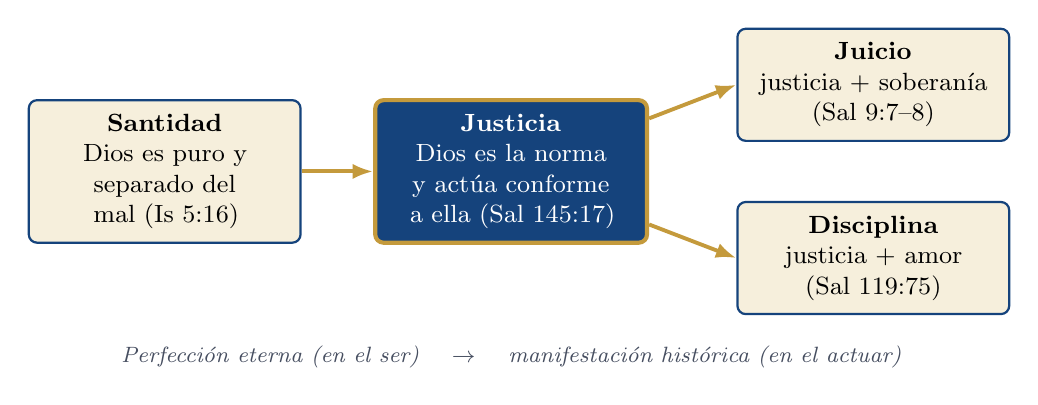
\begin{tikzpicture}[font=\small,
  c/.style={draw=azul,line width=0.8pt,fill=papiro,rounded corners=3pt,text width=3.1cm,align=center,inner sep=5pt},
  d/.style={draw=dorado,line width=1.5pt,fill=azul,text=white,rounded corners=3pt,text width=3.1cm,align=center,inner sep=5pt},
  f/.style={-{Latex[length=2.6mm]},dorado,line width=1.4pt}]
\node[c] (s) at (0,0) {\textbf{Santidad}\\ Dios es puro y separado del mal (Is 5:16)};
\node[d] (j) at (4.4,0) {\textbf{Justicia}\\ Dios es la norma y actúa conforme a ella (Sal 145:17)};
\node[c] (ju) at (9.0,1.1) {\textbf{Juicio}\\ justicia + soberanía (Sal 9:7--8)};
\node[c] (di) at (9.0,-1.1) {\textbf{Disciplina}\\ justicia + amor (Sal 119:75)};
\draw[f] (s)--(j); \draw[f] (j)--(ju.west); \draw[f] (j)--(di.west);
\node[font=\footnotesize\itshape,text=gris] at (4.4,-2.35) {Perfección eterna (en el ser) \quad $\rightarrow$ \quad manifestación histórica (en el actuar)};
\end{tikzpicture}\par
{\footnotesize\color{gris}\textit{Figura 2.} La justicia entre la santidad y el juicio. \textit{Nota.} Elaboración propia a partir del esquema del autor de la serie.}
\end{center}

Isaías une los dos primeros eslabones en un solo verso: ``\SENOR{} de los ejércitos será exaltado en juicio, y el Dios Santo será santificado con justicia'' (\heb{וְהָאֵל הַקָּדוֹשׁ נִקְדָּשׁ בִּצְדָקָה}, Is 5:16). El Santo se muestra santo haciendo justicia. Pink cita a Charnock en la misma línea: ``Su justicia es una justicia santa'' (Pink, 2020, cap. 8).

\subsection{Las distinciones de la teología}
La teología sistemática ha ordenado el atributo con algunas distinciones clásicas. Berkhof (1938/1996) distingue la \emph{justicia rectoral}, por la que Dios establece un gobierno moral y leyes justas, y la \emph{justicia distributiva}, por la que ejecuta esas leyes; esta última es \emph{remunerativa} cuando premia y \emph{retributiva} cuando castiga. La Biblia da textos para cada una:

\begin{center}\small\renewcommand{\arraystretch}{1.2}
\begin{tabular}{@{}L{3.3cm}L{5.5cm}L{5.6cm}@{}}
\toprule
\textbf{Aspecto} & \textbf{Qué significa} & \textbf{Textos} \\ \midrule
En su ser & Dios es recto; no hay en él injusticia & Dt 32:4; Sal 92:15; Ro 9:14 \\
Legislativa & Da leyes justas, reflejo de su carácter & Dt 4:8; Sal 19:9; Ro 7:12 \\
Retributiva & Paga a cada uno según sus obras & Job 34:11; Ro 2:5--6; 2 Ts 1:6 \\
Remunerativa & Recompensa conforme a su promesa & He 6:10; 2 Ti 4:8 \\
Defensora & Hace justicia al oprimido & Dt 10:18; Sal 103:6; 146:7 \\
Salvadora & Cumple su pacto y libera & Jue 5:11; Is 46:13; Sal 98:2 \\
\bottomrule
\end{tabular}\par
{\footnotesize\color{gris}\textit{Tabla 5.} Aspectos de la justicia de Dios. \textit{Nota.} Las cuatro primeras filas siguen las distinciones clásicas (Berkhof, 1938/1996); las dos últimas recogen el uso hebreo estudiado en la sección anterior.}
\end{center}

Las dos últimas filas corrigen una visión parcial. Si la justicia de Dios fuera solo retributiva, sería una mala noticia para todos; pero en la Biblia hebrea la justicia de Dios es, con mucha frecuencia, la razón de la esperanza del oprimido.

\subsection{Dos niveles: la perfección eterna y la justicia revelada}
La justicia de Dios puede mirarse en dos niveles, y la Escritura los une. En el primero, la justicia es una \destacar{perfección eterna} del ser de Dios: Dios es recto en sí mismo, antes de toda criatura y de toda ley escrita (Dt 32:4; Sal 92:15). En el segundo, esa misma justicia \destacar{baja a la historia} y se deja conocer en palabras concretas: los mandamientos, estatutos, decretos y testimonios que Dios dio a su pueblo. La ley no es una norma exterior que Dios inventó para otros; es su propia justicia puesta por escrito. Un verso del Salmo 119 junta los dos niveles en una sola línea:

\hebverso{צִדְקָתְךָ צֶדֶק לְעוֹלָם וְתוֹרָתְךָ אֱמֶת}
\begin{cita}Tu justicia es justicia eterna, y tu ley la verdad.\fuente{(Sal 119:142)}\end{cita}

La primera mitad mira al ser de Dios: su justicia es \emph{tsedeq le'olam}, ``justicia para siempre''. La segunda mira a lo que Dios dio: \emph{toratjá emet}, ``tu ley es verdad''. La justicia eterna de Dios tiene una forma visible en la tierra, y esa forma es su Torá. La sección siguiente desarrolla ese segundo nivel.

\begin{center}
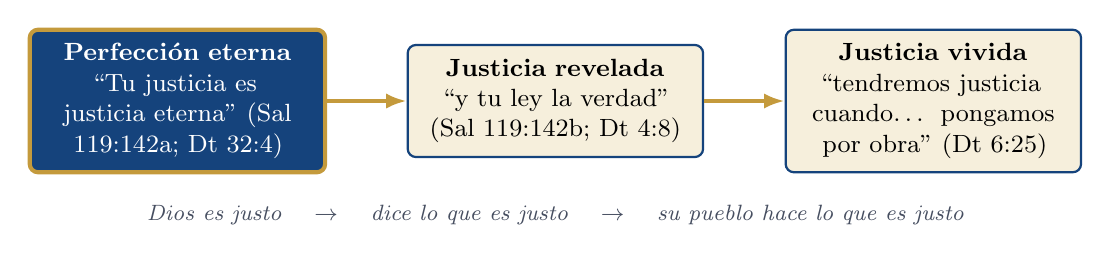
\begin{tikzpicture}[font=\small,
  c/.style={draw=azul,line width=0.8pt,fill=papiro,rounded corners=3pt,text width=3.4cm,align=center,inner sep=5pt},
  d/.style={draw=dorado,line width=1.5pt,fill=azul,text=white,rounded corners=3pt,text width=3.4cm,align=center,inner sep=5pt},
  f/.style={-{Latex[length=2.6mm]},dorado,line width=1.4pt}]
\node[d] (e) at (0,0) {\textbf{Perfección eterna}\\ ``Tu justicia es justicia eterna'' (Sal 119:142a; Dt 32:4)};
\node[c] (l) at (4.8,0) {\textbf{Justicia revelada}\\ ``y tu ley la verdad'' (Sal 119:142b; Dt 4:8)};
\node[c] (v) at (9.6,0) {\textbf{Justicia vivida}\\ ``tendremos justicia cuando\ldots{} pongamos por obra'' (Dt 6:25)};
\draw[f] (e)--(l); \draw[f] (l)--(v);
\node[font=\footnotesize\itshape,text=gris] at (4.8,-1.45) {Dios es justo \quad $\rightarrow$ \quad dice lo que es justo \quad $\rightarrow$ \quad su pueblo hace lo que es justo};
\end{tikzpicture}\par
{\footnotesize\color{gris}\textit{Figura 3.} Los niveles de la justicia de Dios. \textit{Nota.} Elaboración propia a partir del pedido del autor de la serie.}
\end{center}

\subsection{Definición}
\begin{tcolorbox}[colback=papiro,colframe=azul,boxrule=1pt,arc=3pt]
\textbf{La justicia de Dios} es, en su nivel eterno, la perfección de su ser por la cual él mismo es la norma de todo lo recto (\emph{tsedeq}), y todo lo que hace está en perfecta conformidad con ella. En la Biblia, esa justicia se revela en su \textbf{ley}: sus mandamientos, estatutos, decretos y testimonios son ``justicia eterna'' (Sal 119:142, 144) y ``todos justos'' (Sal 19:9). Conforme a ella Dios juzga sin acepción de personas (\emph{mishpat}), da a cada uno lo que corresponde, defiende al débil y cumple su pacto salvando a su pueblo (\emph{tsedaqá}). ``Justo es \SENOR{} en todos sus caminos'' (Sal 145:17). En Cristo, Dios se mostró ``el justo, y el que justifica'' (Ro 3:26), para que ``la justicia de la ley se cumpliese en nosotros'' (Ro 8:4).
\end{tcolorbox}

\begin{nota}[Precisión]
La definición es síntesis propuesta en este capítulo a partir de la definición de la serie (``Dios es justo en todos sus caminos''), del esquema del autor, de su pedido de ``bajar'' la justicia eterna a las leyes y mandamientos (Sal 19; 119), y de los textos estudiados.
\end{nota}

%===================================================================
\section{La justicia de Dios en su ley}\label{sec:ley-justo}

\subsection{``Tu justicia es justicia eterna'': la estrofa \emph{tsade} del Salmo 119}
El Salmo 119 es el gran acróstico de la ley: 22 estrofas de ocho versos, una por letra, y en cada estrofa los ocho versos empiezan con la misma letra. Como en el Salmo 145, la estrofa de la letra \heb{צ} \emph{tsade} (vv. 137--144) está dedicada a la justicia. Empieza con la misma confesión que el texto ancla:

\hebverso{צַדִּיק אַתָּה יְהוָה וְיָשָׁר מִשְׁפָּטֶיךָ \\ צִוִּיתָ צֶדֶק עֵדֹתֶיךָ וֶאֱמוּנָה מְאֹד}
\begin{cita}Justo eres tú, oh \SENOR, y rectos tus juicios. Tus testimonios, que has recomendado, son rectos y muy fieles.\fuente{(Sal 119:137--138)}\end{cita}

\begin{center}\small\renewcommand{\arraystretch}{1.2}
\begin{tabular}{@{}L{1.4cm}L{5.4cm}L{7.4cm}@{}}
\toprule
\textbf{Verso} & \textbf{RVR1960} & \textbf{Qué dice de la justicia} \\ \midrule
137 & ``Justo eres tú, oh \SENOR, y rectos tus juicios'' & Dios es \emph{tsaddiq}; sus \emph{mishpatim} son rectos: el ser y la ley van juntos. \\
138 & ``Tus testimonios\ldots{} son rectos y muy fieles'' & Hebreo: ``mandaste \emph{tsedeq} tus testimonios'': lo que Dios manda es justicia. \\
142 & ``Tu justicia es justicia eterna, y tu ley la verdad'' & El nivel eterno y el nivel revelado en un solo verso. \\
144 & ``Justicia eterna son tus testimonios'' & Los testimonios tienen la misma eternidad que la justicia de Dios. \\
\bottomrule
\end{tabular}\par
{\footnotesize\color{gris}\textit{Tabla 6.} La estrofa \emph{tsade} del Salmo 119. \textit{Nota.} Elaboración propia; hebreo según la BHS.}
\end{center}

El resto del salmo repite la idea: ``todos tus mandamientos son justicia'' (\heb{כִּי כָל־מִצְוֹתֶיךָ צֶּדֶק}, v. 172); ``la suma de tu palabra es verdad, y eterno es todo juicio de tu justicia'' (\heb{כָּל־מִשְׁפַּט צִדְקֶךָ}, v. 160). Siete veces el salmista habla de ``tus justos juicios'' (\emph{mishpetei tsidqeja}, literalmente ``los juicios de tu justicia''; vv. 7, 62, 106, 160, 164 y otros): ``Siete veces al día te alabo a causa de tus justos juicios'' (v. 164).

\begin{nota}[Precisión]
La correspondencia entre la estrofa \emph{tsade} del Sal 119 y la línea \emph{tsade} del Sal 145 (ambas abren con \emph{tsaddiq}) es observación propia; en los dos acrósticos la palabra que empieza con esa letra es la más natural, ``justo''.
\end{nota}

\subsection{``La ley de \SENOR{} es perfecta'': el Salmo 19}
El Salmo 19 tiene dos partes. La primera canta a Dios en la creación: ``Los cielos cuentan la gloria de Dios'' (v. 1); el sol sale ``como esposo que sale de su tálamo'' (v. 5). La segunda canta a Dios en su ley, con seis líneas construidas igual: un nombre de la ley, ``de \SENOR'', una cualidad y un efecto en el ser humano.

\hebverso{תּוֹרַת יְהוָה תְּמִימָה מְשִׁיבַת נָפֶשׁ עֵדוּת יְהוָה נֶאֱמָנָה מַחְכִּימַת פֶּתִי \\ פִּקּוּדֵי יְהוָה יְשָׁרִים מְשַׂמְּחֵי־לֵב מִצְוַת יְהוָה בָּרָה מְאִירַת עֵינָיִם \\ יִרְאַת יְהוָה טְהוֹרָה עוֹמֶדֶת לָעַד מִשְׁפְּטֵי־יְהוָה אֱמֶת צָדְקוּ יַחְדָּו}
\begin{cita}La ley de \SENOR{} es perfecta, que convierte el alma; el testimonio de \SENOR{} es fiel, que hace sabio al sencillo. Los mandamientos de \SENOR{} son rectos, que alegran el corazón; el precepto de \SENOR{} es puro, que alumbra los ojos. El temor de \SENOR{} es limpio, que permanece para siempre; los juicios de \SENOR{} son verdad, todos justos.\fuente{(Sal 19:7--9 [19:8--10])}\end{cita}

\begin{center}\small\renewcommand{\arraystretch}{1.2}
\begin{tabular}{@{}L{3.3cm}L{2.0cm}L{3.3cm}L{5.4cm}@{}}
\toprule
\textbf{Nombre de la ley} & \textbf{RVR1960} & \textbf{Cualidad} & \textbf{Efecto} \\ \midrule
\heb{תּוֹרָה} \emph{torá} & ley & \heb{תְּמִימָה} perfecta, íntegra & \heb{מְשִׁיבַת נָפֶשׁ} ``hace volver el alma'', la restaura \\
\heb{עֵדוּת} \emph{edut} & testimonio & \heb{נֶאֱמָנָה} fiel, firme & \heb{מַחְכִּימַת פֶּתִי} hace sabio al simple \\
\heb{פִּקּוּדִים} \emph{piqqudim} & mandamientos & \heb{יְשָׁרִים} rectos & \heb{מְשַׂמְּחֵי־לֵב} alegran el corazón \\
\heb{מִצְוָה} \emph{mitsvá} & precepto & \heb{בָּרָה} pura, limpia & \heb{מְאִירַת עֵינָיִם} alumbra los ojos \\
\heb{יִרְאָה} \emph{yir'á} & temor & \heb{טְהוֹרָה} limpio & \heb{עוֹמֶדֶת לָעַד} permanece para siempre \\
\heb{מִשְׁפָּטִים} \emph{mishpatim} & juicios & \heb{אֱמֶת} verdad & \heb{צָדְקוּ יַחְדָּו} ``son justos todos juntos'' \\
\bottomrule
\end{tabular}\par
{\footnotesize\color{gris}\textit{Tabla 7.} Los seis nombres de la ley en el Salmo 19:7--9. \textit{Nota.} Elaboración propia; hebreo según la BHS; sentidos según BDB y HALOT. La RVR1960 traduce \emph{piqqudim} ``mandamientos'' y \emph{mitsvá} ``precepto''.}
\end{center}

\begin{filologia}[Sal 19:7 y 19:9 (19:8 y 19:10 en hebreo)]
\begin{tabular}{@{}L{3.2cm}L{1.6cm}L{10cm}@{}}
\heb{תְּמִימָה} \emph{temimá} & \heb{תמם} & ``perfecta, completa'': la misma raíz de ``la Roca, cuya obra es perfecta'' (\emph{tamim}, Dt 32:4). La ley tiene la perfección de su autor. \\[2pt]
\heb{מְשִׁיבַת נָפֶשׁ} & \heb{שׁוב} & ``que hace volver el alma'': el verbo de la conversión y del regreso; la RVR1960 traduce ``que convierte el alma''. \\[2pt]
\heb{צָדְקוּ יַחְדָּו} \emph{tsadqu yajdav} & \heb{צדק} & ``son justos juntos'', ``todos a una son justos'': el verbo \emph{tsadaq} cierra la serie. Ningún juicio de Dios es injusto, y todos concuerdan entre sí. \\
\end{tabular}
\end{filologia}

La estructura enseña dos cosas. Primero, cada cualidad de la ley es una cualidad de Dios: perfecta como la Roca (Dt 32:4), fiel, recta, pura, verdadera, justa. La ley es un retrato moral de su autor. Segundo, la última palabra es \emph{tsadqu}: la serie de los nombres de la ley termina en la justicia. El salmo vuelve después al tono personal: los juicios son ``deseables\ldots{} más que el oro'' y ``dulces más que miel'' (v. 10), y el salmista pide: ``Líbrame de los que me son ocultos'' (v. 12). La justicia revelada en la ley no aplasta al que la lee: lo atrae y lo examina.

\subsection{El vocabulario de la ley}
La Biblia usa varias palabras para la ley de Dios, y a menudo las pone juntas. Cada una mira la misma voluntad justa desde un ángulo distinto:

\begin{center}\small\renewcommand{\arraystretch}{1.18}
\begin{tabular}{@{}L{2.9cm}L{4.1cm}L{2.7cm}L{1.3cm}L{1.6cm}@{}}
\toprule
\textbf{Término} & \textbf{Sentido de la raíz} & \textbf{RVR1960} & \textbf{AT} & \textbf{Sal 119} \\ \midrule
\heb{תּוֹרָה} \emph{torá} & instrucción, enseñanza (\heb{ירה} ``señalar, enseñar'') & ley & $\approx$220 & 25 \\
\heb{מִצְוָה} \emph{mitsvá} & orden, mandato (\heb{צוה} ``mandar'') & mandamiento, precepto & $\approx$180 & 22 \\
\heb{חֹק}, \heb{חֻקָּה} \emph{joq}, \emph{juqqá} & lo grabado, lo fijado (\heb{חקק} ``grabar'') & estatuto, ordenanza & $\approx$230 & 22 \\
\heb{מִשְׁפָּט} \emph{mishpat} & decisión judicial, derecho (\heb{שׁפט}) & juicio, decreto, derecho & $\approx$420 & 23 \\
\heb{עֵדוּת}, \heb{עֵדָה} \emph{edut}, \emph{edá} & testimonio (\heb{עוד} ``atestiguar'') & testimonio & $\approx$85 & 23 \\
\heb{פִּקּוּדִים} \emph{piqqudim} & encargos, cosas confiadas (\heb{פקד}) & mandamientos & 24 & 21 \\
\heb{מִשְׁמֶרֶת} \emph{mishméret} & lo que se custodia (\heb{שׁמר} ``guardar'') & precepto, ordenanza & $\approx$78 & --- \\
\heb{דָּבָר}, \heb{אִמְרָה} \emph{davar}, \emph{imrá} & palabra, dicho & palabra, dichos & --- & 24; 19 \\
\bottomrule
\end{tabular}\par
{\footnotesize\color{gris}\textit{Tabla 8.} El vocabulario de la ley. \textit{Nota.} Conteo propio por números de Strong en la RVR1960-Strong (H8451, H4687, H2706, H2708, H4941, H5715, H5713, H6490, H4931, H1697, H565); las cifras del AT son aproximadas porque el etiquetado es incompleto. Las del Salmo 119 coinciden con las de los comentarios. Verificar en e-Sword.}
\end{center}

Cuatro de estas palabras aparecen juntas en el encargo de David a Salomón:

\hebverso{לִשְׁמֹר חֻקֹּתָיו מִצְוֹתָיו וּמִשְׁפָּטָיו וְעֵדְוֹתָיו כַּכָּתוּב בְּתוֹרַת מֹשֶׁה}
\begin{cita}Guarda los preceptos de \SENOR{} tu Dios, andando en sus caminos, y observando sus estatutos y mandamientos, sus decretos y sus testimonios, de la manera que está escrito en la ley de Moisés, para que prosperes en todo lo que hagas y en todo aquello que emprendas.\fuente{(1 R 2:3)}\end{cita}

``Andar en sus caminos'' (\heb{לָלֶכֶת בִּדְרָכָיו}) es el lenguaje del Salmo 145:17: Dios es justo ``en todos sus caminos'', y su pueblo anda en esos caminos guardando sus estatutos, mandamientos, decretos y testimonios.

\subsection{``Estatutos y juicios justos''}
Moisés presenta la ley como la justicia de Dios visible ante las naciones:

\hebverso{וּמִי גּוֹי גָּדוֹל אֲשֶׁר־לוֹ חֻקִּים וּמִשְׁפָּטִים צַדִּיקִם כְּכֹל הַתּוֹרָה הַזֹּאת}
\begin{cita}Y ¿qué nación grande hay que tenga estatutos y juicios justos como es toda esta ley que yo pongo hoy delante de vosotros?\fuente{(Dt 4:8)}\end{cita}

Los estatutos son \emph{tsaddiqim}, ``justos'': el mismo adjetivo que el Salmo 145:17 aplica a Dios. Por eso, cuando el hijo pregunte ``¿Qué significan los testimonios y estatutos y decretos?'' (Dt 6:20), el padre debe contar la salida de Egipto y concluir:

\hebverso{וּצְדָקָה תִּהְיֶה־לָּנוּ כִּי־נִשְׁמֹר לַעֲשׂוֹת אֶת־כָּל־הַמִּצְוָה הַזֹּאת}
\begin{cita}Y tendremos justicia cuando cuidemos de poner por obra todos estos mandamientos delante de \SENOR{} nuestro Dios, como él nos ha mandado.\fuente{(Dt 6:25)}\end{cita}

El orden importa: primero la redención (``\SENOR{} nos sacó de Egipto'', v. 21), después los mandamientos, y en ellos la \emph{tsedaqá} del pueblo. La ley no se da para que Israel llegue a ser pueblo de Dios, sino porque ya lo es. Nehemías resume el Sinaí con los adjetivos de la justicia: ``les diste juicios rectos, leyes verdaderas, y estatutos y mandamientos buenos'' (Neh 9:13). E Isaías anuncia que el Siervo traerá la justicia de Dios en la ley: ``\SENOR{} se complació por amor de su justicia en magnificar la ley y engrandecerla'' (Is 42:21).

\subsection{La ley justa, leída con Pablo}
Pablo, que fue ``en cuanto a la justicia que es en la ley, irreprensible'' (Flp 3:6), nunca dice que la ley sea injusta. Al contrario:

\begin{cita}De manera que la ley a la verdad es santa, y el mandamiento santo, justo y bueno.\fuente{(Ro 7:12)}\end{cita}

Los tres adjetivos son los del Salmo 19: santa, justa (\grc{δικαία}), buena. El problema no está en la ley, sino en el ser humano que no puede cumplirla (Ro 7:14; 8:3). Por eso Pablo dice que la fe no anula la ley: ``¿Luego por la fe invalidamos la ley? En ninguna manera, sino que confirmamos la ley'' (Ro 3:31). En Cristo y por el Espíritu, la justicia de la ley llega a cumplirse: Dios envió a su Hijo ``para que la justicia de la ley (\grc{τὸ δικαίωμα τοῦ νόμου}) se cumpliese en nosotros, que no andamos conforme a la carne, sino conforme al Espíritu'' (Ro 8:4). Es la promesa de los profetas: ``Daré mi ley en su mente, y la escribiré en su corazón'' (Jer 31:33); ``pondré dentro de vosotros mi Espíritu, y haré que andéis en mis estatutos'' (Ez 36:27). Y el resumen de toda la ley es el amor: ``el cumplimiento de la ley es el amor'' (Ro 13:10; cf. Gá 5:14). Jesús lo había dicho: ``No he venido para abrogar, sino para cumplir'' (Mt 5:17).

\begin{nota}[Antecedente histórico: cómo el judaísmo organizó la ley]
Lo que sigue no es la justicia de Dios declarada en la Biblia, sino la manera en que la tradición judía posterior organizó los mandamientos, como extensión de lo que entendió por justicia. Se registra solo como antecedente.
\begin{itemize}\setlength{\itemsep}{1pt}
\item \textbf{Halajá} (\heb{הֲלָכָה}, de \heb{הלך} ``andar''): ``el camino por el cual se anda''; primero una decisión legal concreta, luego todo el sistema legal judío. La palabra recoge el lenguaje bíblico de ``andar en sus caminos'' (1 R 2:3).
\item \textbf{Torá oral}: hacia el 200 e.\,c., Rabí Yehudá haNasí compiló la \textbf{Misná}; los sabios la comentaron durante unos 300 años en la \textbf{Guemará}; ambas forman el \textbf{Talmud}.
\item \textbf{613 mandamientos}: Rabí Simlai enseñó que ``613 mandamientos fueron dichos a Moisés: 365 negativos, como los días del año solar, y 248 positivos, como los miembros del cuerpo'' (\emph{Makot} 23b). El mismo pasaje dice que los profetas los resumieron: David en once (Sal 15), Isaías en seis, Miqueas en tres (Mi 6:8), y Habacuc en uno: ``el justo por su fe vivirá'' (Hab 2:4; \emph{Makot} 24a).
\item \textbf{Tres clases de mandamientos} (a partir de Dt 6:20): \emph{mishpatim} (``juicios'': leyes que la razón reconoce, como no matar ni robar), \emph{edot} (``testimonios'': leyes que recuerdan los actos de Dios, como el sábado y las fiestas) y \emph{juqqim} (``estatutos'': leyes que se obedecen sin conocer su razón, como la vaca roja o la mezcla de telas). El Talmud distingue los \emph{mishpatim}, ``que si no estuvieran escritos, sería justo escribirlos'', de los \emph{juqqim}, a los que ``el adversario objeta'' (\emph{Yomá} 67b).
\end{itemize}
Estas clasificaciones son rabínicas y medievales; la Biblia usa los términos juntos y de modo intercambiable (Sal 19; 119; 1 R 2:3), sin un sistema fijo. Fuentes: Talmud de Babilonia (Steinsaltz, 2017). Conviene cotejar \emph{Makot} 23b--24a y \emph{Yomá} 67b en Sefaria.
\end{nota}

%===================================================================
\section{Teología: justicia y misericordia}

\subsection{El trono de Dios}
El material de la serie sobre la sincronía de los atributos cita dos textos del Salterio. El primero describe el trono de Dios:

\hebverso{צֶדֶק וּמִשְׁפָּט מְכוֹן כִּסְאֶךָ חֶסֶד וֶאֱמֶת יְקַדְּמוּ פָנֶיךָ}
\begin{cita}Justicia y juicio son el cimiento de tu trono; misericordia y verdad van delante de tu rostro.\fuente{(Sal 89:14 [89:15])}\end{cita}

\begin{filologia}[Sal 89:14 (89:15)]
\begin{tabular}{@{}L{3.2cm}L{1.6cm}L{10cm}@{}}
\heb{מְכוֹן כִּסְאֶךָ} \emph{mejon kis'ejá} & \heb{כון} & ``el fundamento de tu trono'': la base firme sobre la que se asienta. \\[2pt]
\heb{יְקַדְּמוּ פָנֶיךָ} \emph{yeqaddemu fanéja} & \heb{קדם} & ``van delante de tu rostro'': como heraldos que preceden al rey. \\
\end{tabular}
\end{filologia}

La imagen ordena los atributos sin enfrentarlos. La justicia y el juicio son el cimiento; la misericordia y la verdad son los heraldos que salen al encuentro de las personas. El trono no descansa en la misericordia a costa de la justicia, ni en la justicia sin misericordia. El mismo verso se repite casi literal en el Salmo 97:2: ``Nubes y oscuridad alrededor de él; justicia y juicio son el cimiento de su trono''.

\subsection{``La justicia y la paz se besaron''}
El segundo texto describe un encuentro:

\hebverso{חֶסֶד־וֶאֱמֶת נִפְגָּשׁוּ צֶדֶק וְשָׁלוֹם נָשָׁקוּ}
\begin{cita}La misericordia y la verdad se encontraron; la justicia y la paz se besaron. La verdad brotará de la tierra, y la justicia mirará desde los cielos.\fuente{(Sal 85:10--11 [85:11--12])}\end{cita}

El Salmo 85 es una oración del pueblo que volvió del exilio y aún no ve restaurada la tierra (vv. 1--7). Los atributos aparecen personificados: se encuentran y se besan. La justicia ``mira desde los cielos'' (\heb{נִשְׁקָף}), inclinada sobre la tierra. El material de la serie lee en este salmo la clave de la cruz: allí ``la Justicia fue satisfecha, la Misericordia fue derramada y la Santidad fue vindicada''.

\begin{nota}[Precisión]
La lectura del Salmo 85:10 como profecía de la cruz es tipológica y es la del material del autor de la serie; en su contexto el salmo pide la restauración de Israel tras el exilio. El Midrash leyó el mismo verso como una disputa entre los atributos en la creación del ser humano (\emph{Bereshit Rabá} 8:5), texto ya visto en el capítulo sobre la verdad.
\end{nota}

\subsection{``De ningún modo tendrá por inocente''}
La revelación del Nombre en el Sinaí pone en una misma frase el perdón y la justicia: Dios es el ``que perdona la iniquidad, la rebelión y el pecado, y que de ningún modo tendrá por inocente al malvado'' (Éx 34:7). La ley exige lo mismo a los jueces: ``no matarás al inocente y justo; porque yo no justificaré al impío'' (\heb{כִּי לֹא־אַצְדִּיק רָשָׁע}, Éx 23:7). Y Proverbios lo hace principio: ``El que justifica al impío, y el que condena al justo, ambos son igualmente abominación a \SENOR'' (Pr 17:15).

\begin{filologia}[Éx 23:7; Pr 17:15]
\begin{tabular}{@{}L{3.2cm}L{1.6cm}L{10cm}@{}}
\heb{לֹא־אַצְדִּיק רָשָׁע} & \heb{צדק} & ``no declararé justo al impío'': hifil de \emph{tsadaq}, el verbo forense ``declarar justo, absolver''. \\[2pt]
\heb{מַצְדִּיק רָשָׁע} \emph{matsdiq rashá} & \heb{צדק} & ``el que declara justo al impío'': el mismo hifil, en participio. \\
\end{tabular}
\end{filologia}

Aquí está el nudo que el Antiguo Testamento deja abierto. Si Dios perdona al culpable, ¿no hace lo que él mismo prohíbe? Pablo escribirá que Dios es ``aquel que justifica al impío'' (Ro 4:5), con las mismas palabras de Proverbios en griego. Cómo puede Dios hacerlo sin dejar de ser justo es la pregunta que responde Romanos 3:21--26 (sección~\ref{sec:cristo-justo}).

\subsection{Pink: la justicia en los demás atributos}
Pink no dedica un capítulo a la justicia, pero la trata en varios. En la santidad: ``Dios se negaría a Sí mismo, deshonraría sus perfecciones, si considerara justo y santo lo que no lo es en sí mismo'' (2020, cap. 8). En la misericordia: ``La misericordia de Dios nunca se muestra si perjudica su santidad y justicia'' y ``Dios no será injusto consigo mismo'' (cap. 14). En la gracia: ``Si el pecador insiste en recibir pura justicia, entonces el Lago de Fuego debe ser su porción eterna'' (cap. 13). En la fidelidad, enseña a decir con Daniel en la disciplina: ``Tuya es, Señor, la justicia, y nuestra la confusión de rostro'' (Dn 9:7; cap. 10). Y en la soberanía advierte que, al pensar en el dominio absoluto de Dios, ``nunca debemos perder de vista sus perfecciones morales. Dios es justo y bueno, y siempre hace lo correcto'' (cap. 19).

El hilo es constante: en Pink, la justicia es el límite que ningún otro atributo cruza. La misericordia no la anula, la gracia no la burla, la soberanía no la contradice.

%===================================================================
\section{``¿Dónde está el Dios de justicia?''}

\subsection{La justicia puesta a prueba}
La Biblia no esconde que la justicia de Dios es, a veces, difícil de ver. Los mismos libros que la afirman registran la protesta de los justos. Jeremías la formula ante Dios:

\hebverso{צַדִּיק אַתָּה יְהוָה כִּי אָרִיב אֵלֶיךָ אַךְ מִשְׁפָּטִים אֲדַבֵּר אוֹתָךְ}
\begin{cita}Justo eres tú, oh \SENOR, para que yo dispute contigo; sin embargo, alegaré mi causa ante ti. ¿Por qué es prosperado el camino de los impíos, y tienen bien todos los que se portan deslealmente?\fuente{(Jer 12:1)}\end{cita}

\begin{filologia}[Jer 12:1]
\begin{tabular}{@{}L{3.2cm}L{1.6cm}L{10cm}@{}}
\heb{צַדִּיק אַתָּה} \emph{tsaddiq atá} & \heb{צדק} & ``justo eres tú'': la misma confesión del Sal 119:137. \\[2pt]
\heb{כִּי אָרִיב} \emph{ki ariv} & \heb{ריב} & ``cuando entablo pleito'': \emph{riv} es el lenguaje del tribunal. \\[2pt]
\heb{מִשְׁפָּטִים אֲדַבֵּר} & \heb{שׁפט} & ``hablaré juicios contigo'': presentaré el caso. \\
\end{tabular}
\end{filologia}

El profeta no niega la justicia de Dios: parte de ella. Porque Dios es justo, Jeremías puede llevarle su caso. La queja de los justos en la Biblia no es incredulidad; es apelar a Dios contra la apariencia de las cosas.

\subsection{Habacuc: ``el justo por su fe vivirá''}
Habacuc hace la misma pregunta dos veces. Primero sobre la injusticia en Judá: ``la ley es debilitada, y el juicio no sale según la verdad; por cuanto el impío asedia al justo, por eso sale torcida la justicia'' (Hab 1:4). Después, cuando Dios anuncia que usará a Babilonia para castigar a Judá, sobre el instrumento del castigo:

\begin{cita}Muy limpio eres de ojos para ver el mal, ni puedes ver el agravio; ¿por qué ves a los menospreciadores, y callas cuando destruye el impío al más justo que él?\fuente{(Hab 1:13)}\end{cita}

La respuesta de Dios no explica todo. Manda escribir una visión que ``aunque tardare, espéralo'' (2:3), y da una frase que marcará la historia:

\hebverso{הִנֵּה עֻפְּלָה לֹא־יָשְׁרָה נַפְשׁוֹ בּוֹ וְצַדִּיק בֶּאֱמוּנָתוֹ יִחְיֶה}
\begin{cita}He aquí que aquel cuya alma no es recta, se enorgullece; mas el justo por su fe vivirá.\fuente{(Hab 2:4)}\end{cita}

\begin{filologia}[Hab 2:4]
\begin{tabular}{@{}L{3.2cm}L{1.6cm}L{10cm}@{}}
\heb{לֹא־יָשְׁרָה} \emph{lo-yashrá} & \heb{ישׁר} & ``no es recta'': el soberbio, cuyo interior está torcido. \\[2pt]
\heb{וְצַדִּיק} \emph{vetsaddiq} & \heb{צדק} & ``pero el justo'': el que pertenece al pacto y espera en Dios. \\[2pt]
\heb{בֶּאֱמוּנָתוֹ} \emph{be'emunató} & \heb{אמן} & ``por su fidelidad'', ``por su firmeza'': \emph{emuná} es la fe que se mantiene firme. \\[2pt]
\heb{יִחְיֶה} \emph{yijyé} & \heb{חיה} & ``vivirá'': sobrevivirá al juicio que viene. \\
\end{tabular}
\end{filologia}

La respuesta al problema de la justicia no es una teoría, sino una manera de vivir: el justo vive esperando con fidelidad que Dios cumpla la visión. Pablo citará este verso como texto clave de la justicia de Dios (Ro 1:17; Gá 3:11).

\begin{nota}[Precisión textual]
El hebreo dice ``por \emph{su} fe'' (la del justo); la Septuaginta, \grc{ὁ δὲ δίκαιος ἐκ πίστεώς μου ζήσεται}, ``por \emph{mi} fidelidad'' (la de Dios); Pablo cita sin pronombre: \grc{ὁ δὲ δίκαιος ἐκ πίστεως ζήσεται} (Ro 1:17). En Qumrán, el comentario a Habacuc (1QpHab VII--VIII) aplica el verso a los que cumplen la Torá y son fieles al Maestro de Justicia.
\end{nota}

\subsection{El Salmo 73: entrar en el santuario}
Asaf confiesa que casi cae al ver ``la prosperidad de los impíos'' (Sal 73:3). Lo resolvió en un lugar: ``Cuando pensé para saber esto, fue duro trabajo para mí, hasta que entrando en el santuario de Dios, comprendí el fin de ellos'' (73:16--17). La justicia de Dios se ve desde el final de la historia, no desde la mitad.

\subsection{Reconocer la justicia en la disciplina}
Hay una segunda manera de enfrentar la justicia de Dios: confesarla cuando el castigo cae sobre uno mismo. Las grandes oraciones del exilio y del regreso lo hacen así:

\hebverso{לְךָ אֲדֹנָי הַצְּדָקָה וְלָנוּ בֹּשֶׁת הַפָּנִים}
\begin{cita}Tuya es, Señor, la justicia, y nuestra la confusión de rostro, como en el día de hoy lleva todo hombre de Judá, los moradores de Jerusalén, y todo Israel, los de cerca y los de lejos, en todas las tierras adonde los has echado a causa de su rebelión con que se rebelaron contra ti.\fuente{(Dn 9:7)}\end{cita}
\begin{cita}Pero tú eres justo en todo lo que ha venido sobre nosotros; porque rectamente has hecho, mas nosotros hemos hecho lo malo.\fuente{(Neh 9:33)}\end{cita}

Daniel y Nehemías no piden a Dios que deje de ser justo; apelan a su misericordia sin negar su justicia: ``no elevamos nuestros ruegos ante ti confiados en nuestras justicias, sino en tus muchas misericordias'' (Dn 9:18). Dios responde a Job con una pregunta que corrige toda queja que se vuelve acusación: ``¿Invalidarás tú también mi juicio? ¿Me condenarás a mí, para justificarte tú?'' (Job 40:8).

%===================================================================
\section{La justicia que defiende al débil}

La justicia de Dios tiene una dirección preferente en la Biblia hebrea: los que no tienen quien los defienda. Moisés la describe en el mismo verso que proclama la grandeza de Dios:

\hebverso{עֹשֶׂה מִשְׁפַּט יָתוֹם וְאַלְמָנָה וְאֹהֵב גֵּר לָתֶת לוֹ לֶחֶם וְשִׂמְלָה}
\begin{cita}Porque \SENOR{} vuestro Dios es Dios de dioses y Señor de señores, Dios grande, poderoso y temible, que no hace acepción de personas, ni toma cohecho; que hace justicia al huérfano y a la viuda; que ama también al extranjero dándole pan y vestido.\fuente{(Dt 10:17--18)}\end{cita}

\begin{filologia}[Dt 10:17--18]
\begin{tabular}{@{}L{3.2cm}L{1.6cm}L{10cm}@{}}
\heb{לֹא־יִשָּׂא פָנִים} \emph{lo-yissá fanim} & \heb{נשׂא} & ``no levanta rostros'': no hace acepción de personas, no favorece al importante. \\[2pt]
\heb{וְלֹא יִקַּח שֹׁחַד} & \heb{לקח} & ``ni toma soborno''. \\[2pt]
\heb{עֹשֶׂה מִשְׁפַּט} \emph{osé mishpat} & \heb{שׁפט} & ``hace el derecho'' del huérfano y la viuda: les da lo que les corresponde. \\
\end{tabular}
\end{filologia}

Los Salmos lo repiten como un estribillo: ``\SENOR{} es el que hace justicia y derecho a todos los que padecen violencia'' (Sal 103:6); ``que hace justicia a los agraviados, que da pan a los hambrientos'' (Sal 146:7). En el Salmo 82, Dios se levanta en la asamblea de los poderosos y los acusa: ``¿Hasta cuándo juzgaréis injustamente\ldots? Defended al débil y al huérfano; haced justicia al afligido y al menesteroso'' (Sal 82:2--3).

Jeremías llega a definir el conocimiento de Dios por la justicia social. Del buen rey Josías dice:

\hebverso{דָּן דִּין־עָנִי וְאֶבְיוֹן אָז טוֹב הֲלוֹא־הִיא הַדַּעַת אֹתִי נְאֻם־יְהוָה}
\begin{cita}El juzgó la causa del afligido y del menesteroso, y entonces estuvo bien. ¿No es esto conocerme a mí? dice \SENOR.\fuente{(Jer 22:16)}\end{cita}

La frase final, ``¿no es esto conocerme?'', retoma Jeremías 9:24. Conocer al Dios que hace justicia es hacer justicia. Por eso la justicia es comunicable: ``Oh hombre, él te ha declarado lo que es bueno, y qué pide \SENOR{} de ti: solamente hacer justicia, y amar misericordia, y humillarte ante tu Dios'' (Mi 6:8). Y por eso la Torá manda a los jueces: ``La justicia, la justicia seguirás'' (\heb{צֶדֶק צֶדֶק תִּרְדֹּף}, Dt 16:20).

%===================================================================
\section{Un encuentro en la historia de Israel: Abraham ante Sodoma}\label{sec:abraham-justo}

\subsection{``Haciendo justicia y juicio''}
La primera vez que aparece el par \emph{tsedaqá umishpat} en la Biblia, no describe a Dios sino a la familia de Abraham. Antes de destruir Sodoma, Dios delibera consigo mismo:

\hebverso{לְמַעַן אֲשֶׁר יְצַוֶּה אֶת־בָּנָיו וְאֶת־בֵּיתוֹ אַחֲרָיו \\ וְשָׁמְרוּ דֶּרֶךְ יְהוָה לַעֲשׂוֹת צְדָקָה וּמִשְׁפָּט}
\begin{cita}Porque yo sé que mandará a sus hijos y a su casa después de sí, que guarden el camino de \SENOR, haciendo justicia y juicio, para que haga venir \SENOR{} sobre Abraham lo que ha hablado acerca de él.\fuente{(Gn 18:19)}\end{cita}

``El camino del \SENOR'' (\heb{דֶּרֶךְ יְהוָה}) es hacer justicia y juicio. Es el lenguaje del Salmo 145:17: los ``caminos'' de Dios son justos, y su pueblo debe andar en ellos. Dios revela a Abraham lo que va a hacer porque Abraham tiene que aprender cómo juzga Dios para enseñarlo a sus hijos.

\subsection{La pregunta de Abraham}
Dios anuncia que ``descenderá'' a ver si el ``clamor'' (\heb{זַעֲקָה}) contra Sodoma es cierto (18:20--21). La palabra es la del grito de los oprimidos. Abraham se acerca y pregunta:

\hebverso{הַאַף תִּסְפֶּה צַדִּיק עִם־רָשָׁע}
\begin{cita}Y se acercó Abraham y dijo: ¿Destruirás también al justo con el impío?\fuente{(Gn 18:23)}\end{cita}
\hebverso{חָלִלָה לְּךָ מֵעֲשֹׂת כַּדָּבָר הַזֶּה לְהָמִית צַדִּיק עִם־רָשָׁע \\ וְהָיָה כַצַּדִּיק כָּרָשָׁע חָלִלָה לָּךְ הֲשֹׁפֵט כָּל־הָאָרֶץ לֹא יַעֲשֶׂה מִשְׁפָּט}
\begin{cita}Lejos de ti el hacer tal, que hagas morir al justo con el impío, y que sea el justo tratado como el impío; nunca tal hagas. El Juez de toda la tierra, ¿no ha de hacer lo que es justo?\fuente{(Gn 18:25)}\end{cita}

\begin{filologia}[Gn 18:23--25]
\begin{tabular}{@{}L{3.2cm}L{1.6cm}L{10cm}@{}}
\heb{וַיִּגַּשׁ} \emph{vayyiggash} & \heb{נגשׁ} & ``y se acercó'': el verbo de quien se presenta ante un juez o ante el altar. \\[2pt]
\heb{הַאַף תִּסְפֶּה} & \heb{ספה} & ``¿acaso barrerás?'': destruir de una vez, sin distinguir. \\[2pt]
\heb{חָלִלָה לְּךָ} \emph{jalila lejá} & \heb{חלל} & ``¡lejos de ti!'', literalmente ``¡profanación para ti!'': algo indigno de Dios. Se repite dos veces. \\[2pt]
\heb{הֲשֹׁפֵט כָּל־הָאָרֶץ} & \heb{שׁפט} & ``¿el Juez de toda la tierra\ldots?'': primer uso de \emph{shofet} para Dios en la Biblia. \\[2pt]
\heb{לֹא יַעֲשֶׂה מִשְׁפָּט} & \heb{שׁפט} & ``¿no hará juicio (justo)?'': \emph{shofet} y \emph{mishpat}, la misma raíz: el Juez no puede dejar de juzgar con justicia. \\
\end{tabular}
\end{filologia}

La pregunta de Abraham no duda de la justicia de Dios: apela a ella. Abraham conoce un principio que Dios mismo había enseñado en el versículo 19: la justicia distingue entre el justo y el impío. Tratar igual al justo y al impío sería ``profanación''.

\subsection{De cincuenta a diez}
Lo que sigue es una negociación de seis pasos: cincuenta, cuarenta y cinco, cuarenta, treinta, veinte, diez (18:26--32). Abraham insiste con humildad (``he aquí ahora que he comenzado a hablar a mi Señor, aunque soy polvo y ceniza'', v. 27; ``no se enoje ahora mi Señor'', vv. 30, 32), y Dios acepta cada vez. La pregunta de Abraham empezó sobre la justicia (no destruir al justo con el impío) y terminó sobre la misericordia: perdonar a todo el lugar por amor a unos pocos justos (``perdonaré a todo este lugar por amor a ellos'', v. 26).

\begin{center}
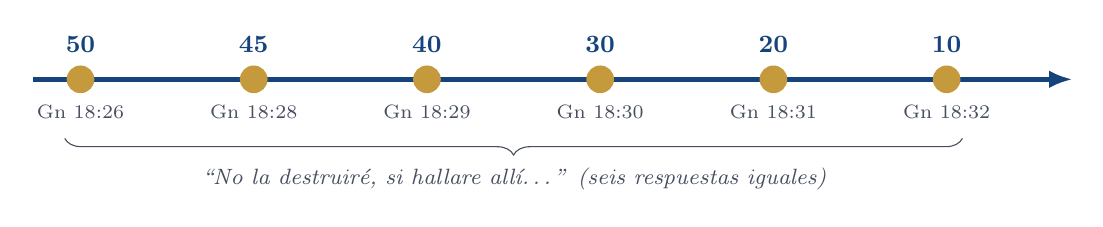
\begin{tikzpicture}[font=\small]
\draw[line width=1.6pt,azul,-{Latex[length=3mm]}] (0,0)--(13.2,0);
\foreach \x/\n/\v in {0.6/50/18:26, 2.8/45/18:28, 5.0/40/18:29, 7.2/30/18:30, 9.4/20/18:31, 11.6/10/18:32}{
 \fill[dorado] (\x,0) circle (5pt);
 \node[above=6pt,font=\small\bfseries,text=azul] at (\x,0) {\n};
 \node[below=6pt,font=\scriptsize,text=gris] at (\x,0) {Gn \v};}
\draw[decorate,decoration={brace,amplitude=6pt,mirror},gris] (0.4,-0.75)--(11.8,-0.75) node[midway,below=7pt,font=\footnotesize\itshape,text=gris] {``No la destruiré, si hallare allí\ldots{}'' (seis respuestas iguales)};
\end{tikzpicture}\par
{\footnotesize\color{gris}\textit{Figura 4.} La intercesión de Abraham por Sodoma. \textit{Nota.} Elaboración propia.}
\end{center}

\subsection{El resultado}
No había diez justos. Pero el relato muestra que la justicia de Dios no destruyó al justo con el impío: ``cuando destruyó Dios las ciudades de la llanura, Dios se acordó de Abraham, y envió fuera a Lot de en medio de la destrucción'' (Gn 19:29). El Juez de toda la tierra hizo justicia en las dos direcciones: juzgó a Sodoma y libró a Lot.

El Nuevo Testamento recoge la misma lectura: Dios ``condenó por destrucción a las ciudades de Sodoma y de Gomorra'' y ``libró al justo Lot'' (2 P 2:6--7). Y Jesús lleva la escena al juicio final: ``en el día del juicio, será más tolerable el castigo para la tierra de Sodoma, que para ti'' (Mt 11:24). La justicia de Dios mide la responsabilidad según la luz recibida.

\begin{nota}[Precisión]
La lectura de Gn 18 como paso ``de la justicia a la misericordia'' es propia; la relación entre el v. 19 (la misión de Abraham) y el v. 25 (su pregunta) es observación frecuente en los comentarios (p. ej., Wenham, 1994).
\end{nota}

\subsection{``Guardó mis mandamientos'': la justicia de Abraham}
La historia de Abraham muestra los dos niveles de la justicia en una sola vida. Cuando Dios renueva la promesa a Isaac, da la razón por la que bendijo a su padre:

\hebverso{עֵקֶב אֲשֶׁר־שָׁמַע אַבְרָהָם בְּקֹלִי \\ וַיִּשְׁמֹר מִשְׁמַרְתִּי מִצְוֹתַי חֻקּוֹתַי וְתוֹרֹתָי}
\begin{cita}por cuanto oyó Abraham mi voz, y guardó mi precepto, mis mandamientos, mis estatutos y mis leyes.\fuente{(Gn 26:5)}\end{cita}

\begin{filologia}[Gn 26:5]
\begin{tabular}{@{}L{3.2cm}L{1.6cm}L{10cm}@{}}
\heb{עֵקֶב אֲשֶׁר} \emph{éqev asher} & \heb{עקב} & ``por cuanto'', ``a consecuencia de que'': la bendición es el fruto de la obediencia. \\[2pt]
\heb{שָׁמַע בְּקֹלִי} & \heb{שׁמע} & ``oyó mi voz'': escuchar y obedecer (cf. Gn 22:18). \\[2pt]
\heb{מִשְׁמַרְתִּי} \emph{mishmartí} & \heb{שׁמר} & ``mi custodia'', lo que se me debe guardar: RVR1960 ``mi precepto''. \\[2pt]
\heb{מִצְוֹתַי} \emph{mitsvotai} & \heb{צוה} & ``mis mandamientos''. \\[2pt]
\heb{חֻקּוֹתַי} \emph{juqqotai} & \heb{חקק} & ``mis estatutos'', lo fijado. \\[2pt]
\heb{תוֹרֹתָי} \emph{torotai} & \heb{ירה} & ``mis instrucciones'', ``mis leyes'' (plural). \\
\end{tabular}
\end{filologia}

Es la primera vez que la Biblia reúne cuatro de los nombres de la ley, y lo hace antes del Sinaí. Abraham no tenía la Torá escrita, pero ``oyó la voz'' de Dios y la guardó. Leídos en orden, los textos de Génesis forman un recorrido:

\begin{center}\small\renewcommand{\arraystretch}{1.2}
\begin{tabular}{@{}L{2.0cm}L{5.4cm}L{6.8cm}@{}}
\toprule
\textbf{Texto} & \textbf{RVR1960} & \textbf{Qué muestra} \\ \midrule
Gn 15:6 & ``creyó a \SENOR, y le fue contado por justicia'' & La justicia de Abraham empieza en la fe: Dios se la cuenta. \\
Gn 18:19 & ``que guarden el camino de \SENOR, haciendo justicia y juicio'' & La justicia recibida se vuelve misión: enseñarla a sus hijos. \\
Gn 18:25 & ``El Juez de toda la tierra, ¿no ha de hacer lo que es justo?'' & Abraham conoce la justicia de Dios y apela a ella. \\
Gn 22:18 & ``por cuanto obedeciste a mi voz'' & La fe probada se muestra en obediencia. \\
Gn 26:5 & ``guardó mi precepto, mis mandamientos, mis estatutos y mis leyes'' & Dios resume la vida de Abraham como obediencia a su ley. \\
\bottomrule
\end{tabular}\par
{\footnotesize\color{gris}\textit{Tabla 10.} La justicia de Abraham en Génesis. \textit{Nota.} Elaboración propia.}
\end{center}

Pablo y Santiago leen la misma historia desde dos lados. Pablo subraya el comienzo: la fe ``le fue contada por justicia'' cuando aún no estaba circuncidado (Ro 4:9--11), y ``no por la ley fue dada a Abraham o a su descendencia la promesa\ldots{} sino por la justicia de la fe'' (Ro 4:13), porque la ley vino ``cuatrocientos treinta años después'' (Gá 3:17). Santiago subraya el fruto: ``la fe actuó juntamente con sus obras, y la fe se perfeccionó por las obras. Y se cumplió la Escritura que dice: Abraham creyó a Dios, y le fue contado por justicia'' (Stg 2:22--23). Génesis 26:5 contiene las dos cosas: Abraham ``oyó la voz'' (fe) y ``guardó'' (obediencia). La justicia de Dios, contada al creyente, produce una vida que guarda sus mandamientos.

\begin{nota}[Precisión]
La tradición rabínica leyó Gn 26:5 como prueba de que Abraham cumplió toda la Torá antes de que fuera dada (\emph{Yomá} 28b); Rashi asigna a cada término una categoría posterior de la ley (decretos rabínicos, mandamientos morales, estatutos sin razón explicada, Torá oral). Rashbam, Ibn Ezra y Ramban leen el verso en un sentido más general, como obediencia a lo que Dios le había mandado. Aquí se sigue el sentido literal del texto; la lectura rabínica es antecedente histórico.
\end{nota}

%===================================================================
\section{La justicia en el judaísmo}\label{sec:judaismo-justo}

\begin{nota}[Precisión]
Esta sección recoge cómo la tradición judía ha leído el atributo. Las fuentes son interpretaciones (litúrgicas, talmúdicas, midrásicas o filosóficas) y se citan según Sefaria y otras ediciones indicadas; la traducción al español es propia.
\end{nota}

\subsection{El salmo de cada día}
El Salmo 145 es la oración que más veces reza un judío. Se recita tres veces al día, dos en el servicio de la mañana y una en el de la tarde, precedido de dos versos que le dan su nombre popular, \emph{Ashré} (Sal 84:4 [84:5]; 144:15). El Talmud lo explica así: ``Todo el que dice \emph{Tehillá leDavid} cada día tres veces tiene asegurado que es hijo del mundo venidero'' (\emph{Berajot} 4b). La razón que da el Talmud es que el salmo reúne el orden alfabético y el verso ``Abres tu mano, y colmas de bendición a todo ser viviente'' (v. 16). El versículo 17, la justicia de Dios en todos sus caminos, es parte de esa oración diaria.

\subsection{``Rey que ama la justicia y el derecho''}
La oración central del judaísmo, la \emph{Amidá}, pide en su undécima bendición la restauración de los jueces de Israel y termina con un título de Dios:

\hebverso{בָּרוּךְ אַתָּה יְהוָה מֶלֶךְ אוֹהֵב צְדָקָה וּמִשְׁפָּט}

``Bendito eres tú, \SENOR, Rey que ama la justicia y el derecho'' (cf. Sal 33:5). El Talmud establece que en los diez días que van de Rosh Hashaná a Yom Kipur la fórmula cambia: ``Todo el año la persona reza \emph{el Dios santo} y \emph{Rey que ama la justicia y el derecho}, excepto en los diez días\ldots{} en que reza \emph{el Rey santo} y \emph{el Rey del juicio}'' (\heb{הַמֶּלֶךְ הַמִּשְׁפָּט}, \emph{Berajot} 12b). En los días del juicio, Dios no es solo el que ama el derecho: es el Derecho mismo.

\subsection{``Si quieres un mundo, no hay juicio estricto''}
El Midrash comenta la pregunta de Abraham con una paradoja atribuida a Rabí Leví:

\hebverso{אִם עוֹלָם אַתָּה מְבַקֵּשׁ אֵין דִּין \\ וְאִם דִּין אַתָּה מְבַקֵּשׁ אֵין עוֹלָם}

``Si quieres un mundo, no hay juicio (estricto); y si quieres juicio, no hay mundo. ¿Por qué tomas la cuerda por los dos extremos? Quieres el mundo y quieres el juicio'' (\emph{Bereshit Rabá} 39:6; cf. 49:9). Abraham pone a Dios ante el problema que la Escritura dejó abierto en Éxodo 34:7: un juicio sin misericordia acabaría con el mundo. La tradición respondió con la doctrina de las dos medidas, \emph{middat haddín} y \emph{middat harajamim}, que Rashi encuentra ya en Génesis 1:1: Dios ``asoció'' la misericordia a la justicia para que el mundo pudiera subsistir.

\begin{nota}[Precisión]
El dicho de Rabí Leví aparece en \emph{Bereshit Rabá} 39:6 y, con variantes, en 49:9, aplicado en ambos casos a Gn 18:25. Conviene cotejar el texto completo en Sefaria.
\end{nota}

\subsection{\emph{Tsidduq haddín}: justificar el juicio}
El judaísmo dio forma litúrgica a la confesión de Daniel y Nehemías. Ante una mala noticia, la Misná manda bendecir: \heb{בָּרוּךְ דַּיַּן הָאֱמֶת} \emph{barukh dayyán ha'emet}, ``Bendito el Juez de la verdad'' (\emph{Misná Berajot} 9:2); y añade que ``uno está obligado a bendecir por el mal como bendice por el bien'' (9:5). Esta bendición se dice hasta hoy al recibir la noticia de una muerte.

El Talmud cuenta el martirio de Rabí Janiná ben Teradión, condenado por los romanos por enseñar la Torá, junto con la condena de su esposa y de su hija:

\hebverso{בְּשָׁעָה שֶׁיָּצְאוּ שְׁלָשְׁתָּן צִדְּקוּ עֲלֵיהֶם אֶת הַדִּין}

``Cuando salieron los tres, justificaron el juicio sobre sí''. Él dijo: ``Él es la Roca, cuya obra es perfecta'' (Dt 32:4a); su esposa: ``Dios de verdad, y sin ninguna iniquidad en él; es justo y recto'' (Dt 32:4b); su hija: ``grande en consejo y magnífico en hechos; porque tus ojos están abiertos sobre todos los caminos de los hijos de los hombres'' (Jer 32:19) (\emph{Avodá Zará} 18a). De aquí recibe su nombre la oración fúnebre \emph{Tsidduq haddín}, ``justificación del juicio'', que comienza con Deuteronomio 32:4.

\begin{nota}[Precisión]
El nombre y el uso fúnebre de \emph{Tsidduq haddín} pertenecen a la liturgia posterior al Talmud; el relato de \emph{Avodá Zará} 18a es su fuente tradicional. El texto de la Misná Berajot 9:2 y 9:5 conviene cotejarlo en Sefaria.
\end{nota}

\subsection{El juez, socio de Dios}
El Talmud eleva la tarea del juez humano: ``Todo juez que juzga un juicio de verdad conforme a su verdad, aunque sea una sola hora, la Escritura lo considera como si se hubiera hecho socio del Santo, bendito sea, en la obra de la creación'' (\emph{Shabat} 10a). Y sobre ``la justicia, la justicia seguirás'' (Dt 16:20), enseña que la repetición incluye tanto el juicio como el acuerdo justo entre las partes, y manda buscar el mejor tribunal (\emph{Sanedrín} 32b). La justicia humana es comunicada: participa del orden que Dios estableció.

\subsection{\emph{Tsedaqá}: la justicia que se da}
En el hebreo posbíblico, \emph{tsedaqá} pasó a significar sobre todo ``limosna, caridad''. El cambio ya se insinúa en el arameo de Daniel, que aconseja a Nabucodonosor: ``tus pecados redime con justicia, y tus iniquidades haciendo misericordias para con los oprimidos'' (\heb{וַחֲטָיָךְ בְּצִדְקָה פְרֻק}, Dn 4:27 [4:24]). Proverbios 10:2, ``la justicia libra de muerte'', se leyó en el Talmud como ``la caridad libra de muerte'' (\emph{Shabat} 156b).

Maimónides explica la palabra así: \emph{tsedaqá} ``deriva de \emph{tsedeq}, justicia; denota el acto de dar a cada uno lo que le corresponde'', y se usa también para los deberes que la conciencia moral impone hacia el prójimo, ``como cuando curamos la herida del que sufre'' (\emph{Guía de los perplejos} III, 53). Para la tradición judía, dar al pobre no es generosidad opcional: es justicia.

\subsection{Qumrán: ``mi justificación está en la justicia de Dios''}
La comunidad de Qumrán tenía un fundador al que llamaba \heb{מוֹרֵה הַצֶּדֶק} \emph{Moré hatsédeq}, ``el Maestro de Justicia'' (CD I, 11; 1QpHab). En el himno final de la \emph{Regla de la Comunidad}, un miembro confiesa:

\begin{cita}En cuanto a mí, si tropiezo, las misericordias de Dios serán mi salvación eterna. Si caigo por el pecado de la carne, mi justificación estará en la justicia de Dios, que permanece para siempre\ldots{} Me juzgará en la justicia de su verdad, y en la grandeza de su bondad perdonará todos mis pecados.\fuente{(1QS XI, 12--14)}\end{cita}

El texto es notable porque, antes de Pablo, un judío confiesa que su ``justificación'' (\heb{מִשְׁפָּטִי} \emph{mishpatí}, ``mi juicio'') descansa en la \heb{צִדְקַת אֵל} \emph{tsidqat El}, ``la justicia de Dios'', no en sí mismo. Otro texto de Qumrán, la carta llamada 4QMMT, cierra con una frase que retoma Génesis 15:6: ``y te será contado por justicia al hacer lo recto y lo bueno delante de él''.

\begin{nota}[Precisión]
1QS según la traducción inglesa de Vermes (2004), en versión propia al español; cotejar con García Martínez (1992) y con la Leon Levy Dead Sea Scrolls Digital Library. 4QMMT C 31 según la edición de Qimron y Strugnell (1994). La relación de estos textos con Pablo se discute: en Qumrán la justicia de Dios sostiene a quien guarda la Torá según la interpretación de la comunidad; en Pablo se recibe ``aparte de la ley'' (Ro 3:21).
\end{nota}

%===================================================================
\section{La justicia de Dios en Cristo, leída con Pablo}\label{sec:cristo-justo}

\subsection{``Irreprensible en cuanto a la justicia''}
Pablo era un judío formado en las Escrituras de Israel. De su vida anterior dice: ``en cuanto a la justicia que es en la ley, irreprensible'' (Flp 3:6). Era el lenguaje del Salmo 145 y de Qumrán: un hombre que buscaba andar en ``los caminos'' de Dios. El encuentro con ``el Justo'' (Hch 22:14) cambió el lugar de esa justicia:

\begin{cita}Y ciertamente, aun estimo todas las cosas como pérdida por la excelencia del conocimiento de Cristo Jesús, mi Señor, por amor del cual lo he perdido todo, y lo tengo por basura, para ganar a Cristo, y ser hallado en él, no teniendo mi propia justicia, que es por la ley, sino la que es por la fe de Cristo, la justicia que es de Dios por la fe.\fuente{(Flp 3:8--9)}\end{cita}

\begin{filologia}[Flp 3:9]
\begin{tabular}{@{}L{3.2cm}L{1.6cm}L{10cm}@{}}
\grc{ἐμὴν δικαιοσύνην} & \grc{δίκη} & ``mi (propia) justicia'': la que nace de la ley. \\[2pt]
\grc{τὴν ἐκ θεοῦ δικαιοσύνην} & \grc{δίκη} & ``la justicia (que viene) de Dios'': la preposición \grc{ἐκ} indica origen. \\[2pt]
\grc{ἐπὶ τῇ πίστει} & \grc{πίστις} & ``sobre la base de la fe''. \\
\end{tabular}
\end{filologia}

\subsection{``La justicia de Dios se revela''}
Romanos, la carta de la justicia de Dios, enuncia su tema al comienzo:

\begin{cita}Porque no me avergüenzo del evangelio, porque es poder de Dios para salvación a todo aquel que cree; al judío primeramente, y también al griego. Porque en el evangelio la justicia de Dios se revela por fe y para fe, como está escrito: Mas el justo por la fe vivirá.\fuente{(Ro 1:16--17)}\end{cita}

Tres textos del Antiguo Testamento convergen aquí. ``Salvación'' y ``justicia'' juntas, reveladas, ``al judío\ldots{} y al griego'': es el Salmo 98:2 en griego, \grc{ἐγνώρισεν κύριος τὸ σωτήριον αὐτοῦ ἐναντίον τῶν ἐθνῶν, ἀπεκάλυψεν τὴν δικαιοσύνην αὐτοῦ}. ``No me avergüenzo'' recuerda Isaías 28:16 (citado en Ro 9:33; 10:11). Y ``el justo por la fe vivirá'' es Habacuc 2:4: la respuesta que Dios dio al profeta que preguntaba por su justicia.

\begin{center}\small\renewcommand{\arraystretch}{1.2}
\begin{tabular}{@{}L{2.4cm}L{4.4cm}L{4.4cm}L{3.4cm}@{}}
\toprule
\textbf{Texto} & \textbf{Hebreo (TM)} & \textbf{Septuaginta} & \textbf{Pablo} \\ \midrule
Sal 98:2 & \heb{גִּלָּה צִדְקָתוֹ} ``reveló su justicia'' & \grc{ἀπεκάλυψεν τὴν δικαιοσύνην αὐτοῦ} & \grc{δικαιοσύνη θεοῦ\ldots{} ἀποκαλύπτεται} (Ro 1:17) \\
Hab 2:4 & \heb{וְצַדִּיק בֶּאֱמוּנָתוֹ יִחְיֶה} & \grc{ὁ δὲ δίκαιος ἐκ πίστεώς μου ζήσεται} & \grc{ὁ δὲ δίκαιος ἐκ πίστεως ζήσεται} (Ro 1:17) \\
Sal 143:2 & \heb{לֹא־יִצְדַּק לְפָנֶיךָ כָל־חָי} & \grc{οὐ δικαιωθήσεται ἐνώπιόν σου πᾶς ζῶν} & \grc{οὐ δικαιωθήσεται πᾶσα σὰρξ ἐνώπιον αὐτοῦ} (Ro 3:20) \\
Gn 15:6 & \heb{וַיַּחְשְׁבֶהָ לּוֹ צְדָקָה} & \grc{ἐλογίσθη αὐτῷ εἰς δικαιοσύνην} & igual (Ro 4:3; Gá 3:6) \\
\bottomrule
\end{tabular}\par
{\footnotesize\color{gris}\textit{Tabla 9.} Los textos del Antiguo Testamento detrás de la ``justicia de Dios'' en Pablo. \textit{Nota.} TM según la BHS; LXX de Rahlfs-Hanhart; NA28. El eco del Sal 98:2 en Ro 1:17 es señalado por Hays (1989).}
\end{center}

\begin{nota}[Precisión]
Qué significa ``justicia de Dios'' (\grc{δικαιοσύνη θεοῦ}) en Pablo es una de las discusiones centrales de la teología del Nuevo Testamento. Para la lectura de la Reforma, es la justicia que Dios \emph{da} al creyente (genitivo de origen; cf. Flp 3:9). Käsemann (1969) la entendió como el poder salvador de Dios que reclama al mundo; Wright (2013), como la fidelidad de Dios a su pacto con Israel; Moo (1996) sostiene que en Ro 1:17 incluye a la vez la actividad de Dios y el don que resulta de ella. La lectura hebrea estudiada en este capítulo (\emph{tsedaqá} como acción que salva y como norma) explica por qué las tres lecturas encuentran apoyo.
\end{nota}

\subsection{``El justo, y el que justifica''}
El centro de la enseñanza de Pablo sobre la justicia de Dios está en Romanos 3. Pablo ha mostrado que ``no hay justo, ni aun uno'' (3:10, a partir del Sal 14:1--3) y que ``por las obras de la ley ningún ser humano será justificado delante de él'' (3:20, Sal 143:2). Entonces escribe:

\begin{cita}Pero ahora, aparte de la ley, se ha manifestado la justicia de Dios, testificada por la ley y por los profetas; la justicia de Dios por medio de la fe en Jesucristo, para todos los que creen en él. Porque no hay diferencia, por cuanto todos pecaron, y están destituidos de la gloria de Dios, siendo justificados gratuitamente por su gracia, mediante la redención que es en Cristo Jesús, a quien Dios puso como propiciación por medio de la fe en su sangre, para manifestar su justicia, a causa de haber pasado por alto, en su paciencia, los pecados pasados, con la mira de manifestar en este tiempo su justicia, a fin de que él sea el justo, y el que justifica al que es de la fe de Jesús.\fuente{(Ro 3:21--26)}\end{cita}

\begin{filologia}[Ro 3:25--26]
\begin{tabular}{@{}L{3.2cm}L{1.6cm}L{10cm}@{}}
\grc{ἱλαστήριον} \emph{hilastērion} & \grc{ἱλάσκομαι} & ``propiciación'': en la LXX, la tapa del arca, el \emph{kapporet} que se rociaba en Yom Kipur (Éx 25:17; Lv 16:14). \\[2pt]
\grc{εἰς ἔνδειξιν τῆς δικαιοσύνης αὐτοῦ} & \grc{ἐνδείκνυμι} & ``para demostración de su justicia'': la frase se repite dos veces (vv. 25 y 26). \\[2pt]
\grc{διὰ τὴν πάρεσιν} & \grc{παρίημι} & ``a causa del dejar pasar'' los pecados anteriores: Dios no los había castigado plenamente. \\[2pt]
\grc{δίκαιον καὶ δικαιοῦντα} & \grc{δίκη} & ``justo y justificador'': adjetivo y participio de la misma raíz, unidos por ``y''. \\
\end{tabular}
\end{filologia}

Pablo responde aquí la pregunta que dejaron abierta Éxodo 34:7, Éxodo 23:7 y Proverbios 17:15. Dios había ``pasado por alto'' los pecados del pasado, y eso ponía en duda su justicia: un juez que absuelve al culpable es abominación. En la cruz, Dios trató el pecado con toda seriedad, y por eso puede justificar al que cree sin dejar de ser justo. Las dos palabras que la Biblia hebrea parecía oponer, ``justo'' y ``que declara justo'', quedan unidas por un ``y'' (\grc{καί}): \grc{δίκαιον καὶ δικαιοῦντα}.

El paralelo más cercano es Isaías 45:21: \emph{El tsaddiq umoshía}, ``Dios justo y Salvador''. Lo que Isaías dijo con dos palabras, justicia y salvación, Pablo lo dice con dos palabras de la misma raíz.

\begin{nota}[Precisión]
La conexión entre Ro 3:26 e Is 45:21 es una lectura propuesta por varios comentaristas, no una cita explícita; la LXX de Is 45:21 dice \grc{δίκαιος καὶ σωτήρ}. La paradoja de Pr 17:15 frente a Ro 4:5 (\grc{τὸν δικαιοῦντα τὸν ἀσεβῆ}) se comenta desde antiguo; el material de la serie la resume: ``en la cruz se reunieron la santidad, la justicia y el amor''.
\end{nota}

\subsection{``Lo hizo pecado\ldots{} para que fuésemos justicia de Dios''}
Pablo formula el intercambio en una frase:

\begin{cita}Al que no conoció pecado, por nosotros lo hizo pecado, para que nosotros fuésemos hechos justicia de Dios en él.\fuente{(2 Co 5:21)}\end{cita}

El ``Justo'' tomó el lugar del injusto. Pedro lo dice con las palabras de este capítulo: ``Cristo padeció una sola vez por los pecados, el justo por los injustos, para llevarnos a Dios'' (1 P 3:18). Es el lenguaje del Siervo de Isaías: ``por su conocimiento justificará mi siervo justo a muchos, y llevará las iniquidades de ellos'' (\heb{יַצְדִּיק צַדִּיק עַבְדִּי לָרַבִּים}, Is 53:11).

\subsection{``Justicia nuestra'': Jeremías en Corinto}
En 1 Corintios, Pablo cita expresamente el verso clave de esta serie. Los corintios se jactaban de sabiduría y de linaje; Pablo responde:

\begin{cita}Mas por él estáis vosotros en Cristo Jesús, el cual nos ha sido hecho por Dios sabiduría, justificación, santificación y redención; para que, como está escrito: El que se gloría, gloríese en el Señor.\fuente{(1 Co 1:30--31)}\end{cita}

``El que se gloría, gloríese en el Señor'' es el resumen de Jeremías 9:23--24. Jeremías decía que el sabio no se gloríe en su sabiduría, sino en conocer al \SENOR{} que hace misericordia, juicio y justicia. Pablo dice que Cristo ``nos ha sido hecho'' sabiduría y justicia (\grc{δικαιοσύνη}). La justicia que Jeremías atribuía a Dios, y que en 23:6 ponía en el nombre del Mesías, ``\SENOR, justicia nuestra'', Pablo la encuentra en Cristo.

\begin{nota}[Precisión]
La cita de Jer 9:24 en 1 Co 1:31 es explícita (``como está escrito''). La relación entre ``nos ha sido hecho\ldots{} justicia'' (1 Co 1:30) y \emph{YHWH tsidqenu} (Jer 23:6) es lectura propia; la tradición cristiana la hizo desde antiguo.
\end{nota}

\subsection{El justo juicio de Dios}
La justicia de Dios en Cristo no elimina el juicio: lo confirma. Pablo habla del ``día de la ira y de la revelación del justo juicio de Dios (\grc{δικαιοκρισίας}), el cual pagará a cada uno conforme a sus obras'' (Ro 2:5--6, citando Sal 62:12 y Pr 24:12), porque ``no hay acepción de personas para con Dios'' (Ro 2:11), el principio de Deuteronomio 10:17. En Atenas anuncia que Dios ``ha establecido un día en el cual juzgará al mundo con justicia, por aquel varón a quien designó'' (Hch 17:31): la frase \grc{κρίνειν τὴν οἰκουμένην ἐν δικαιοσύνῃ} es la de los Salmos 9:8; 96:13 y 98:9 en la Septuaginta. El Juez de toda la tierra (Gn 18:25) juzgará por medio de Cristo.

Ante la objeción ``¿Qué, pues, diremos? ¿Que hay injusticia en Dios?'', Pablo responde: ``En ninguna manera'' (Ro 9:14). Y al final de su vida espera ``la corona de justicia, la cual me dará el Señor, juez justo, en aquel día'' (2 Ti 4:8).

\begin{nota}[Precisión]
La autoría paulina de 2 Timoteo se discute; la idea tiene respaldo en cartas indiscutidas (Ro 2:5--11; 2 Co 5:10). Hch 17:31 es un discurso de Pablo según Lucas.
\end{nota}

\subsection{La justicia de Dios, cumplida en Cristo}
Leída con Pablo, la justicia de Dios se cumple en Cristo en cinco afirmaciones: en el evangelio ``la justicia de Dios se revela'' (Ro 1:17); en la cruz Dios es ``el justo, y el que justifica'' (Ro 3:26); en Cristo los creyentes son ``hechos justicia de Dios'' (2 Co 5:21); Cristo ``nos ha sido hecho\ldots{} justificación'' para que nos gloriemos en el Señor (1 Co 1:30--31); y Dios ``juzgará al mundo con justicia'' por medio de él (Hch 17:31). Pablo lee el ``justo es \SENOR{} en todos sus caminos'' del Salmo 145 a la luz del camino de Cristo, en quien ``habita corporalmente toda la plenitud de la Deidad'' (Col 2:9). En él, la justicia y la paz se besaron: ``Justificados, pues, por la fe, tenemos paz para con Dios por medio de nuestro Señor Jesucristo'' (Ro 5:1).

%===================================================================
\section{Aplicación: vivir ante el Dios justo}

``Dios es justo en todos sus caminos''. La frase de la serie tiene consecuencias concretas.

\begin{enumerate}
\item \textbf{Confiar en el Juez.} Hay injusticias que ningún tribunal humano reparará. La pregunta de Abraham es también una certeza: ``El Juez de toda la tierra, ¿no ha de hacer lo que es justo?'' (Gn 18:25). Por eso Pablo manda: ``No os venguéis vosotros mismos, amados míos, sino dejad lugar a la ira de Dios; porque escrito está: Mía es la venganza, yo pagaré, dice el Señor'' (Ro 12:19, citando Dt 32:35). Y Jesús promete: ``¿Y acaso Dios no hará justicia a sus escogidos, que claman a él día y noche?'' (Lc 18:7).

\item \textbf{Llevarle la queja.} La fe bíblica no prohíbe preguntar. Jeremías dijo ``Justo eres tú'' y luego presentó su caso (Jer 12:1); Habacuc preguntó ``¿hasta cuándo?'' (Hab 1:2). El creyente puede hacer lo mismo, siempre que la queja sea una apelación a Dios y no una acusación contra él (Job 40:8), y que espere el final, como Asaf, ``en el santuario'' (Sal 73:17).

\item \textbf{Reconocer su justicia en la disciplina.} Cuando el mal que sufrimos es consecuencia de nuestro pecado, la respuesta es la de Daniel: ``Tuya es, Señor, la justicia, y nuestra la confusión de rostro'' (Dn 9:7). Pink la recomienda: ``en lugar de murmurar, le agradecemos por ello'' (2020, cap. 10). El salmista lo había aprendido: ``Conozco, oh \SENOR, que tus juicios son justos, y que conforme a tu fidelidad me afligiste'' (Sal 119:75).

\item \textbf{Vivir de la justicia recibida.} Nadie puede presentarse ante Dios con ``su propia justicia'' (Flp 3:9); ``todas nuestras justicias'' son ``como trapo de inmundicia'' (Is 64:6). El evangelio no rebaja la justicia de Dios: la cumple en Cristo. El creyente descansa en ``\SENOR, justicia nuestra'' (Jer 23:6), y puede decir con Pablo: ``¿Quién acusará a los escogidos de Dios? Dios es el que justifica'' (Ro 8:33).

\item \textbf{Amar su ley.} Si la ley es la justicia de Dios puesta por escrito, leerla es conocerlo. ``En la ley de \SENOR{} está su delicia, y en su ley medita de día y de noche'' (Sal 1:2); sus juicios son ``dulces más que miel'' (Sal 19:10). El creyente no la usa para justificarse, sino para andar en los caminos del Dios justo (1 R 2:3), con la ley escrita en el corazón (Jer 31:33).

\item \textbf{Hacer justicia.} La justicia es comunicable. El que conoce al Dios justo usa balanzas exactas (Lv 19:36), no hace acepción de personas (Lv 19:15; Stg 2:1), defiende al huérfano y a la viuda (Is 1:17) y juzga la causa del pobre, porque ``¿no es esto conocerme a mí?'' (Jer 22:16). Jesús llama bienaventurados a ``los que tienen hambre y sed de justicia'' (Mt 5:6), y Juan concluye: ``Si sabéis que él es justo, sabed también que todo el que hace justicia es nacido de él'' (1 Jn 2:29).
\end{enumerate}

%===================================================================
\section{Síntesis}

``Justo es \SENOR{} en todos sus caminos, y misericordioso en todas sus obras'' (Sal 145:17). Dios es justo en su ser: él es la norma de todo lo recto, y no hay en él injusticia (Dt 32:4). Esa justicia eterna se revela en su ley: ``Tu justicia es justicia eterna, y tu ley la verdad'' (Sal 119:142); sus juicios ``son verdad, todos justos'' (Sal 19:9), y Abraham la guardó (Gn 26:5). Es justo en su actuar: legisla con rectitud, juzga sin acepción de personas, defiende al débil y cumple su pacto salvando a su pueblo (Dt 10:18; Sal 98:2). Su justicia camina con su misericordia, como el cimiento y los heraldos de un mismo trono (Sal 89:14). En Cristo, ``\SENOR, justicia nuestra'' (Jer 23:6), Dios se mostró ``el justo, y el que justifica'' (Ro 3:26).

\begin{center}\small\renewcommand{\arraystretch}{1.18}
\begin{tabular}{@{}L{2.4cm}L{11.4cm}@{}}
\toprule
\textbf{Mirada} & \textbf{Aporte al atributo} \\ \midrule
Hebrea & \emph{tsaddiq} y \emph{jasid} en paralelo (Sal 145:17); la justicia eterna revelada en la ley (Sal 119:142; Sal 19:7--9; Dt 4:8; 6:25); Abraham guardó sus mandamientos (Gn 26:5); \emph{tsedeq} como norma (balanzas, sendas); \emph{tsedaqá umishpat}; las ``justicias'' que salvan (Jue 5:11); la defensa del débil (Dt 10:18); el Juez de toda la tierra (Gn 18:25); el lamento que apela (Jer 12:1; Hab 2:4). \\
Judía & El \emph{Ashré} diario (\emph{Berajot} 4b); ``Rey que ama la justicia y el derecho'' (\emph{Berajot} 12b); ``si quieres un mundo, no hay juicio estricto'' (\emph{Bereshit Rabá} 39:6); \emph{tsidduq haddín} (\emph{Avodá Zará} 18a); el juez socio de Dios (\emph{Shabat} 10a); \emph{tsedaqá} como caridad (Maimónides); Qumrán (1QS XI). \\
Pink & La justicia como límite de los demás atributos: santa (cap. 8), no anulada por la misericordia (cap. 14) ni por la gracia (cap. 13), reconocida en la disciplina (cap. 10). \\
Paulina & La ley santa, justa y buena (Ro 7:12) cumplida en el Espíritu (Ro 8:4); la justicia de Dios revelada en el evangelio (Ro 1:17); el justo y el que justifica (Ro 3:26); el intercambio (2 Co 5:21); Cristo hecho justicia (1 Co 1:30--31, con Jer 9:24); el justo juicio (Ro 2:5; Hch 17:31). \\
\bottomrule
\end{tabular}\end{center}

\begin{cita}Mas alábese en esto el que se hubiere de alabar: en entenderme y conocerme, que yo soy \SENOR, que hago misericordia, juicio y justicia en la tierra; porque estas cosas quiero, dice \SENOR.\fuente{(Jer 9:24 [9:23])}\end{cita}

Conocer al Dios justo no es temer a un tribunal sin rostro, sino conocer al que Abraham interpeló, al que Jeremías llevó su causa, al que Daniel confesó en el exilio y al que, en Cristo, ``justifica al impío'' sin dejar de ser justo.

%===================================================================
\section*{Glosario}
\begin{description}\setlength{\itemsep}{2pt}
\item[\emph{Dikaiokrisía}] (\grc{δικαιοκρισία}). ``Justo juicio'' de Dios (Ro 2:5).
\item[\emph{Dikaiosýnē}] (\grc{δικαιοσύνη}). Justicia; traduce \emph{tsedaqá} y \emph{tsedeq} en la LXX (Ro 1:17).
\item[\emph{Dikaióō}] (\grc{δικαιόω}). Justificar, declarar justo (Ro 3:26; 4:5).
\item[\emph{Díkaios}] (\grc{δίκαιος}). Justo; ``el Justo'', título de Cristo (Hch 3:14).
\item[\emph{Din}] (\heb{דִּין}). Juicio, derecho; \emph{middat haddín}, la medida de la justicia.
\item[\emph{Edut}, \emph{edot}] (\heb{עֵדוּת}). Testimonio(s) de Dios (Sal 19:7; 119:144).
\item[\emph{Joq}, \emph{juqqim}] (\heb{חֹק}). Estatuto, lo fijado (Gn 26:5; Dt 4:8).
\item[\emph{Mitsvá}] (\heb{מִצְוָה}). Mandamiento, precepto (Sal 19:8; 119:172).
\item[\emph{Hilastērion}] (\grc{ἱλαστήριον}). Propiciación; la tapa del arca en la LXX (Ro 3:25).
\item[\emph{Jasid}] (\heb{חָסִיד}). Leal, fiel en amor; ``misericordioso'' (Sal 145:17).
\item[\emph{Mishpat}] (\heb{מִשְׁפָּט}). Juicio, derecho, decisión justa (Gn 18:25; Dt 32:4).
\item[\emph{Piqqudim}] (\heb{פִּקּוּדִים}). Encargos, mandamientos (Sal 19:8).
\item[\emph{Shofet}] (\heb{שֹׁפֵט}). Juez; ``el Juez de toda la tierra'' (Gn 18:25).
\item[\emph{Tsaddiq}] (\heb{צַדִּיק}). Justo (Sal 145:17; Hab 2:4).
\item[\emph{Tsadaq}, hifil \emph{hitsdiq}] (\heb{הִצְדִּיק}). Declarar justo, absolver (Éx 23:7; Is 53:11).
\item[\emph{Tsedaqá}] (\heb{צְדָקָה}). Justicia; acto justo o salvador; en el hebreo posterior, caridad.
\item[\emph{Tsedeq}] (\heb{צֶדֶק}). Justicia, lo exacto, lo correcto (Lv 19:36; Dt 16:20).
\item[\emph{Tsidduq haddín}] (\heb{צִדּוּק הַדִּין}). ``Justificación del juicio'': aceptar el juicio de Dios como justo (\emph{Avodá Zará} 18a).
\item[\emph{Torá}] (\heb{תּוֹרָה}). Instrucción, ley (Sal 19:7; 119:142).
\item[\emph{Tsidqot YHWH}] (\heb{צִדְקוֹת יְהוָה}). ``Las justicias del \SENOR'': sus actos de salvación (Jue 5:11).
\item[\emph{YHWH tsidqenu}] (\heb{יְהוָה צִדְקֵנוּ}). ``El \SENOR, justicia nuestra'' (Jer 23:6).
\end{description}

\section*{Referencias}
\refapa{Bauer, W., Danker, F.~W., Arndt, W.~F., \& Gingrich, F.~W. (2000). \emph{A Greek-English lexicon of the New Testament and other early Christian literature} (3.ª ed.). University of Chicago Press.}
\refapa{Berkhof, L. (1996). \emph{Systematic theology} (Ed. combinada). Eerdmans. (Obra original publicada en 1938)}
\refapa{\emph{Bereshit Rabá} [8:5; 12:15; 39:6; 49:9]. (s.f.). Sefaria. https://www.sefaria.org}
\refapa{Brown, F., Driver, S.~R., \& Briggs, C.~A. (1906). \emph{A Hebrew and English lexicon of the Old Testament}. Clarendon Press.}
\refapa{Elliger, K., \& Rudolph, W. (Eds.). (1997). \emph{Biblia Hebraica Stuttgartensia} (5.ª ed.). Deutsche Bibelgesellschaft.}
\refapa{García Martínez, F. (1992). \emph{Textos de Qumrán}. Trotta.}
\refapa{Hays, R.~B. (1989). \emph{Echoes of Scripture in the letters of Paul}. Yale University Press.}
\refapa{Käsemann, E. (1969). The righteousness of God in Paul. En \emph{New Testament questions of today} (pp.~168--182). SCM Press.}
\refapa{Koehler, L., \& Baumgartner, W. (2001). \emph{The Hebrew and Aramaic lexicon of the Old Testament} (M.~E.~J. Richardson, Trad.; Ed. de estudio). Brill.}
\refapa{Lundbom, J.~R. (2004). \emph{Jeremiah 21--36} (Anchor Bible 21B). Doubleday.}
\refapa{Maimónides. (1903). \emph{The guide for the perplexed} (M. Friedländer, Trad.; 2.ª ed.). Routledge. (Obra original del s.~XII)}
\refapa{\emph{Misná: Berajot} [9:2, 9:5]. (s.f.). Sefaria. https://www.sefaria.org}
\refapa{Moo, D.~J. (1996). \emph{The epistle to the Romans}. Eerdmans.}
\refapa{Nestle, E., \& Aland, K. (Eds.). (2012). \emph{Novum Testamentum Graece} (28.ª ed.). Deutsche Bibelgesellschaft.}
\refapa{Pink, A.~W. (2020). \emph{Los atributos de Dios} (E. Rodríguez Cruz, Trad.). Chapel Library. (Obra original publicada en 1930)}
\refapa{Qimron, E., \& Strugnell, J. (1994). \emph{Qumran Cave 4.V: Miqṣat maʿaśe ha-Torah} (Discoveries in the Judaean Desert 10). Clarendon Press.}
\refapa{Rahlfs, A., \& Hanhart, R. (Eds.). (2006). \emph{Septuaginta} (Ed. rev.). Deutsche Bibelgesellschaft.}
\refapa{Rashi. (s.f.). \emph{Comentario a Génesis} [Gn 1:1]. Sefaria. https://www.sefaria.org}
\refapa{Sanders, J.~A. (1965). \emph{The Psalms Scroll of Qumrân Cave 11 (11QPs\textsuperscript{a})} (Discoveries in the Judaean Desert 4). Clarendon Press.}
\refapa{\emph{Santa Biblia: Reina-Valera 1960}. (1960). Sociedades Bíblicas en América Latina.}
\refapa{\emph{Shemot Rabá} [3:6]. (s.f.). Sefaria. https://www.sefaria.org}
\refapa{\emph{Sidur Ashkenaz} [Amidá; \emph{Ashré}]. (s.f.). Sefaria. https://www.sefaria.org}
\refapa{Steinsaltz, A. (Ed.). (2017). \emph{Koren Talmud Bavli: Edición William Davidson} [Berajot 4b, 12b; Shabat 10a, 156b; Sanedrín 32b; Avodá Zará 18a; Bava Batra 75b; Makot 23b--24a; Yomá 28b, 67b]. Sefaria. https://www.sefaria.org}
\refapa{Strong, J. (1890). \emph{The exhaustive concordance of the Bible}. Hunt \& Eaton.}
\refapa{Vermes, G. (2004). \emph{The complete Dead Sea Scrolls in English} (Ed. rev.). Penguin.}
\refapa{Wenham, G.~J. (1994). \emph{Genesis 16--50} (Word Biblical Commentary 2). Word.}
\refapa{Wright, N.~T. (2013). \emph{Paul and the faithfulness of God}. Fortress Press.}

\end{document}
